\documentclass[12pt,letterpaper, onecolumn]{exam}
\usepackage{amsmath}
\usepackage{amssymb}
\usepackage{tipa}
\usepackage[lmargin=71pt, tmargin=1.2in]
{geometry}  %For centering solution box
%\lhead{Leaft Header\\}
%\rhead{Right Header\\}
% \chead{\hline} % Un-comment to draw line below header
\thispagestyle{empty}   %For removing header/footer from page 1
\usepackage{CJKutf8}
\usepackage{booktabs}
\usepackage{float}
\usepackage{graphicx} 

\newtheorem{remark}{Remark}


\begin{document}

\begingroup  
    \centering
    \LARGE Solutions to "A Practical Guide to Quantitative Finance"\\[0.5em]
    \large \today\\[0.5em]
    \large Huawei Wu\par
\endgroup
\rule{\textwidth}{0.4pt}
\pointsdroppedatright   %Self-explanatory
\printanswers
\renewcommand{\solutiontitle}{\noindent\textbf{Ans:}\enspace}   %Replace "Ans:" with starting keyword in solution box



\section{Probability}

\subsection{Combinatorial Analysis}
\begin{questions}
    \question[1 Mark] (Application Letters) You're sending job applications to 5 firms: Morgan Stanley, Lehman Brothers, UBS, Goldman Sachs, and Merrill Lynch. You have 5 envelopes on the table neatly typed with names and addresses of people at these 5 firms. You even have 5 cover letters personalized to each of these firms. Your 3-year-old tried to be helpful and stuffed each cover letter into each of the envelopes for you. Unfortunately she randomly put letters into envelopes without realizing that the letters are personalized. What is the probability that all 5 cover letters are mailed to the wrong firms?
    
    \begin{solution}
       Let's consider a more general version of the problem. Suppose we have \( n \) envelopes and \( n \) corresponding cover letters, and we number them from left to right as \( 1, 2, \dots, n \) (one, two, up to $n$). A way of placing  these cover letters can be seen as a permutation of these cover letters. The case where no letter is placed in its correct envelope corresponds to a \textbf{derangement}—a permutation with no fixed points.

    \quad There are \( n! \) ($n$ factorial) possible permutations in total. And we use \( D_n \) to denote the number of derangements of the \( n \) cover letters. Let's start with the simplest cases:

\begin{itemize}
    \item When \( n = 1 \), there is only one cover letter, and it is always placed in the correct envelope. So, we have \( D_1 = 0 \).
    \item When \( n = 2 \), the only valid derangement is swapping the two cover letters. So, we have \( D_2 = 1 \).
\end{itemize}

\quad Now, let's consider the general case for \( n \geq 3 \). Since cover letter \( 1 \) cannot be placed in envelope \( 1 \), we have \( n-1 \) choices for where to place it. Suppose we put it in envelope \( k \) (where \( 2 \leq k \leq n \)). Let \( D_{n,k} \) represent the number of derangements where cover letter \( 1 \) is specifically placed in envelope \( k \). Due to symmetry, we know that:

\[
D_{n,2} = D_{n,3} = \dots = D_{n,n}
\]

This means that the total number of derangements of $n$ cover letters can be expressed as:

\[
D_n = (n-1) \cdot D_{n,2}
\]

\quad So, it is enough to analyze \( D_{n,2} \). There are two cases to consider:

\begin{enumerate}
    \item \textbf{Case 1:} Cover letter \( 2 \) is placed in envelope \( 1 \). In this scenario, the remaining elements are cover letters \( 3,4,\dots,n \) and envelopes \( 3,4,\dots,n \). Hence what we need to do next is to permute the remaining $n-2$ cover letters with no fixed points. Consequently, the number of such derangements is $D_{n-2}$.
    \item \textbf{Case 2:} Cover letter \( 2 \) is not placed in envelope \( 1 \). Since the original position of cover letter \( 2 \) (that is, envelope \( 2 \)) has already been taken by cover letter \( 1 \), we can think of envelope \( 1 \) as its new "correct" position. Not placing it there means it is also misplaced, so this situation is equivalent to a derangement of the remaining \( n-1 \) letters, which gives us \( D_{n-1} \).
\end{enumerate}

\quad Thus, we derive the recurrence relation:

\[
D_n = (n-1) \cdot (D_{n-1} + D_{n-2})
\]

This formula allows us to compute the number of derangements recursively. We have 
$$D_3=2\cdot(D_2+D_1)=2\cdot(1+0)=2,$$
$$D_4=3\cdot(D_3+D_2)=3\cdot(2+1)=9,$$
and
$$D_5=4\cdot(D_4+D_3)=4\cdot(9+2)=44.$$
Hence the probability that all 5 cover letters are mailed to the wrong firms is
$$\frac{D_5}{5!}=\frac{44}{120}=\frac{11}{30}.$$
    \end{solution}
    \begin{remark}
        neat \textipa{/ni:t/}, adj. \begin{CJK}{UTF8}{gbsn}整齐的,简洁的\end{CJK}.
    \end{remark}
    
    \question[2 Marks] (Birthday Problem) How many people do we need in a class to make the probability that two people have the same birthday more than $\frac{1}{2}$? (For simplicity, assume $365$ days a year.)
    \begin{solution}
        Assume that there are $n$ people in class. Without any restrictions, we have $365$ possibilities for each one's birthday. The basic principle of counting tells us that there $365^n$ possible ways to assign birthdays to $n$ people.
        
        \quad We want to find the number of ways in which no people share the same birthday. The first person can choose any of the $365$ days as his/her birthday, while the second person must have a different birthday, i.e., he/she has $364$ choices. Generally, for the $r$-th person, there are $365-r+1$ choices. Therefore, the number of ways to assign birthdays to $n$ people such that no people share the same birthday is $365 \times 364 \times \dots \times (365-n+1)$, and the probability that no people share the same birthday is:
        $$\frac{365 \times 364 \times \dots \times (365-n+1)}{365^n}.$$
        We want this probability to be less than $\frac{1}{2}$. The smallest integer $n$ that satisfies this inequality is $23$.
    \end{solution}

    \pagebreak %Not necessary
    
    \question[]($100$-th Digit) What is the $100$-th digit to the right of the decimal point in the decimal representation of $(1+\sqrt{2})^{3000}$?
    \begin{solution}
            Applying the binomial theorem, we have 
            $$(1+\sqrt{2})^n=\sum\limits_{k=0}^n\binom{n}{k}\sqrt{2}^k.$$
            We can divide the above summation into two parts based on whether $k$ is even or odd:
            $$\sum\limits_{k=0}^n\binom{n}{k}\sqrt{2}^k=\sum\limits_{k=2j,0\le j\le\frac{n}{2}}^n\binom{n}{k}\sqrt{2}^k+\sum\limits_{k=2j+1,0\le j\le\frac{n-1}{2}}^n\binom{n}{k}\sqrt{2}^k.$$
            Similarly, we have
            \begin{align*}
                (1-\sqrt{2})^n&=\sum\limits_{k=2j,0\le j\le\frac{n}{2}}^n\binom{n}{k}(-\sqrt{2})^k+\sum\limits_{k=2j+1,0\le j\le\frac{n-1}{2}}^n\binom{n}{k}(-\sqrt{2})^k\\
                &=\sum\limits_{k=2j,0\le j\le\frac{n}{2}}^n\binom{n}{k}\sqrt{2}^k-\sum\limits_{k=2j+1,0\le j\le\frac{n-1}{2}}^n\binom{n}{k}\sqrt{2}^k.
            \end{align*}
            It follows that
            $$(1+\sqrt{2})^n+(1-\sqrt{2})^n=2\cdot\sum\limits_{k=2j,0\le j\le\frac{n}{2}}^n\binom{n}{k}\sqrt{2}^k,$$
            which always a positive integer. Note that $1-\sqrt{2}$ is approximately $0.4$, which implies that
            $$0<(1-\sqrt{2})^{3000}\approx 0.4^{3000}=(0.064)^{1000}<0.1^{1000}=10^{-10000}<10^{-100}.$$
            It follows that the $100$-th digit to the right of the decimal point in the decimal representation of $(1+\sqrt{2})^{3000}$ is $9$.
    \end{solution}

    \question[](Cubic of Integer) Let $x$ be an integer between $1$ and $10^{12}$, what is the probability that the cubic of $x$ ends with $11$.
    \begin{solution}
        We can express $x$ as $x=10b+a$, where $a$ is the last digit of $x$. Applying the binomial theorem, we have 
        $$x^3=(10b+a)^3=1000b^3+300a^2b^2+30a^2b+a^3,$$
        which implies that 
        $$x^3\equiv 30a^2b+a^3\ ({\rm{mod}}\ 100)$$
        and
        $$x^3\equiv a^3\ ({\rm{mod}}\ 10).$$
        Hence the units digit of $x^3$ equals that of $a^3$. Since $0\le a\le 9$, a brute-force search shows that the unit digit of $a^3$ is $1$ if and only if $a=1$. 
        
        \quad If $a=1$, then
        $$x^3\equiv 30b+1\ ({\rm{mod}}\ 100),$$
        which implies that 
        $$\frac{x^3-1}{10}\equiv 3b\ ({\rm{mod}}\ 10).$$
        Note that if the units digit of $x^3$ is $1$, then the tens digit of $x^3$ is equal to the units digit of $\frac{x^3-1}{10}$. Hence the cubic of $x$ ends with $11$ is equivalent to saying that $a=1$ and the units digit of $3b$ is $1$. A brute-force search shows that the latter condition is equivalent to saying that the units digit of $b$ is $7$. Since $x=10b+1$, we conclude that the cubic of $x$ ends with $11$ if and only if the last two digits of $x$ should be $71$, which occurs with probability $\frac{1}{100}$.
    \end{solution}
    \begin{remark}
       $x^3\equiv a^3\ ({\rm{mod}}\ 10)$ can be read as "$x$ cubed in congruent to $a$ cubed modulo $10$".
    \end{remark}
\end{questions}



\subsection{Conditional Probability and Bayes' Formula}

\begin{questions}
    \question[](Boys and Girls) A company is holding a dinner for working mothers with at least one son. 
    \begin{parts}
        \part Ms. Jackson, a mother with two children, is invited. What is the probability that both children are boys?
        \part Your new colleague, Ms. Parker is known to have two children. If you see her walking with one of her children and that child is a boy, what is the probability that both children are boys?
    \end{parts}
    \begin{solution}
        The sample space of the two children is given by 
            $$\Omega=\{(b,b),(b,g),(g,b),(g,g)\}$$
            (e.g., $(g,b)$ means the older child is a girl and the younger child a boy), and each outcome has the same probability of $\frac{1}{4}$.
        \begin{parts}
            \part Since Ms. Jackson is invited, she has at least one son. Let $B$ be the evenet that at least one of the children is a boy and $A$ be the event that both children are boys, we have 
            $$P(A|B)=\frac{P(A\cap B)}{P(B)}=\frac{P\Big(\{(b,b)\}\Big)}{P\Big(\{(b,b),(b,g),(g,b)\}\Big)}=\frac{\frac{1}{4}}{\frac{3}{4}}=\frac{1}{3}.$$
            \part The other child is equally likely to be a boy or a girl (independent of the boy you've seen), so the probability that both children are boys is $\frac{1}{2}$.
        \end{parts}
    \end{solution}

    \question[](All-Girl World?) In a primitive society, every couple prefers to have a baby girl. There is a 50\% chance that each child they have is a girl, and the genders of their children are mutually independent. If each couple insists on having more children until they get a girl and once they have a girl they will stop having more children, what will eventually happen to the fraction of girls in this society?
    \begin{solution}
        Do not let the word “prefer” and a wrong intuition misguide us. The fraction of baby girls are driven by nature, or at least the X and Y chromosomes (\textipa{/"kroUm@s@Um/}), not by the couples’ preference. We only need to look at the key information: 50\% and independence. Every new-born child has equal probability of being a boy or a girl regardless of the gender of any other children. Therefore, a couple having multiple children can be equivalently viewed as multiple couples each having only one child. As a consequence, the fraction of girls born is always 50\% and the fractions of girls in the society will stay stable at 50\%.
    \end{solution}

    \question[](Unfair Coin) You are given 1000 coins. Among them, $1$ coin has heads on both sides. The other $999$ coins are fair coins. You randomly choose a coin and toss it $10$ times. Each time, the coin turns up heads. What is the probability that the coin you choose is the unfair one?

    \begin{solution}
        Let $A$ be the event that the chosen coin is unfair and $B$ be the event that all $10$ tosses are heads. If the coin is fair, each time, the probability of getting a head is $\frac{1}{2}$. If the coin is unfair, the probability of getting a head is $1$. By Bayes' formula, we have
        \begin{align*}
            P(A|B)&=\frac{P(A\cap B)}{P(B)}\\
            &=\frac{P(A)P(B|A)}{P(A)P(B|A)+P(A^c)P(B|A^c)}\\
            &=\frac{\frac{1}{1000}\times 1}{\frac{1}{1000}\times 1+\frac{999}{1000}\times\Big(\frac{1}{2}\Big)^{10}}\\
            &=\frac{2^{10}}{2^{10}+999}\approx 0.506.
        \end{align*}
    \end{solution}
    \begin{remark}
        $A^c$ can be read as "not $A$" or $A$ complement (\textipa{/"kA:mplIment/}), and $P(A|B)$ can be read as "the probability of $A$ given $B$" or "$P$ of $A$ given $B$".
    \end{remark}

    \question[](Fair Probability from an Unfair Coin) If you have an unfair coin, which may bias toward either heads or tails at an unknown probability, can you generate even odds using this coin?
    \begin{solution}
        Assume that the probability of getting heads is $p$. Then the probability of getting tails is $1-p$. Consider two independent tosses. We have four possible outcomes HH, HT, TH and TT with probabilities
        $$\begin{aligned}
            P(HH) &= pp,  & P(HT) &= p(1 - p), \\
            P(TH) &= (1 - p)p,  & P(TT) &= (1 - p)(1 - p).
        \end{aligned}$$
        Hence $P(HT)=P(TH)$. By assigning HT to wining and TH to losing, we can generate even odds.
    \end{solution}

    \question[](Dart Game) Jason throws two darts at a dartboard, aiming for the center. The second dart lands farther from the center than the first. If Jason throws a third dart aiming for the center, what is the probability that the third throw is farther from the center than the first?Assume Jason's skillfulness is constant.
    \begin{solution}        
        We rank the results of the three dart throws based in their distance from the center, from nearest (\textipa{/"nIr@st/}) to farthest (\textipa{/"fA:rDIst/}), as A, B, C. Then there are $6$ possible outcomes with equal probabilities:
            \begin{table}[H]
            \centering
            \begin{tabular}{lcccccc}
                \toprule
                Outcome & 1 & 2 & 3 & 4 & 5 & 6 \\
                \midrule
                1st throw & A & B & A & C & B & C \\
                2nd throw & B & A & C & A & C & B \\
                3rd throw & C & C & B & B & A & A \\
                \bottomrule
            \end{tabular}
        \end{table}
            Let $X$ be the event that the second throw is farther from the center than the first, and $Y$ be the event that the third throw is  from the center than the first. Then the event $X$ consists of outcomes $1$, $3$ and $5$, and the event $XY$ ($X$ and $Y$) consists of $1$ and $3$. Hence we have 
            $$P(Y|X)=\frac{P(XY)}{P(X)}=\frac{\frac{1}{3}}{\frac{1}{2}}=\frac{2}{3}.$$
    \end{solution}

    \question[](Generalized Dart Game) Jason throws $n$ $(n\ge 3)$ darts at a dartboard, aiming for the center. Assume that each subsequent dart is farther from the center than the first dart. If Jason throws a $(n+1)$-th dart aiming for the center, what is the probability that the $(n+1)$-th throw is farther from the center than the first?
    \begin{solution}
        Similarly, we rank the results of the $n+1$ dart throws based in their distance from the center, from nearest to farthest, as $A_1$, $A_2$, $\cdots$, $A_{n+1}$. We can still enumerate all the possible outcomes which have equal probabilities (but we would not actually do it). 
        
        \quad Let $X$ be the event that the subsequent $n-1$ throws are all farther from the center than the first, and $Y$ be the event that the $(n+1)$-th throw is nearer from the center than the first. 
        
        \quad When the event $X$ occurs, either the first throw is the best one, or the first throw is the second best one while the $(n+1)$-th throw is the best one. In other words, the event $X$ consists of the following two types of outcomes:
        \begin{enumerate}
            \item \textbf{Type 1:} The first throw is labelled as $A_1$. At this point, the rankings of the other $n$ throws can be arbitrary. Hence there are $n!$ such outcomes.
            \item \textbf{Type 2:} The first throw is labelled as $A_2$ while the $(n+1)$-th throw is labelled as $A_1$. At this point, the rankings of the other $n-1$ throws can be arbitrary. Hence there are $(n-1)!$ such outcomes.
        \end{enumerate}
         Hence the event $X$ consists of $n!+(n-1)!$ outcomes.

         \quad Similarly, it is easy to see that the event $XY$ consists of the second type of outcomes above, i.e., the event $XY$ consists of $(n-1)!$ outcomes. Therefore, we have 
         $$P(Y|X)=\frac{P(XY)}{P(X)}=\frac{(n-1)!}{n!+(n-1)!}=\frac{1}{n+1}.$$
         The probability that the $(n+1)$-th throw is farther from the center than the first is
         $$P(Y^c|X)=1-P(Y|X)=\frac{n}{n+1}.$$
    \end{solution}

    \question[](Birthday Line) At a movie theater, a whimsical (\textipa{/"wImzIk@l/}, \begin{CJK}{UTF8}{gbsn}古怪的\end{CJK}) manager announces that she will give a free ticket to the first person in line whose birthday is the same as someone who has already bought a ticket. You are given the opportunity to choose any position in line. Assuming that you don't know anyone else's birthday and all birthdays are distributed randomly throughout the year (assuming $365$ days in a year), what position in line gives you the largest chance of getting the free ticket?
\begin{solution}
    Let $A_n$ be the event that the $n$-th person in line gets the free ticket. Then it is clear that the event $A_n$ is equivalent to the event that the first $n-1$ people in line have different birthdays and the $n$-th person has the same birthday as one of the first $n-1$ people. Let $B_{n-1}$ be the event that the first $n-1$ people in line have different birthdays. Then we have 
    $$P(B_{n-1})=\frac{A_{365}^{n-1}}{365^{n-1}}=\frac{365\times 364\times\cdots\times (365-n+2)}{365^{n-1}}.$$
    Let $C_n$ be the event that the $n$-th person has the same birthday as one of the first $n-1$ people. Then we have 
    $$P(C_n|B_{n-1})=\frac{n-1}{365},$$
    that is, we can choose any of the first $n-1$ people's birthdays (which are pairwise distinct) as the $n$-th person's birthday. Hence we have
    \begin{align*}
        P(A_n)&=P(B_{n-1}C_n)=P(B_{n-1})P(C_n|B_{n-1})\\
        &=\frac{365\times 364\times\cdots\times (365-n+2)\times (n-1)}{365^n}.
    \end{align*}
    To determine for which $n$ the probability $P(A_n)$ is maximized, we solve the following system of inequalities:
    $$
    \begin{cases}
        P(A_n)\ge P(A_{n-1}),\Leftrightarrow\frac{A_{365}^{n-1}\times (n-1)}{365^{n-1}}\ge\frac{A_{365}^{n-2}\times (n-2)}{365^{n-2}},\\
        P(A_{n})\ge P(A_{n+1})\Leftrightarrow\frac{A_{365}^{n-1}\times (n-1)}{365^{n-1}}\ge\frac{A_{365}^{n}\times n}{365^n},
    \end{cases}
    $$
    which simplifies to 
    $$
    \begin{cases}
        (365-n+2)(n-1)\ge 365(n-2),\\
        (365-n+1)n\le 365(n-1),
    \end{cases}\Leftrightarrow\begin{cases}
        n^2-3n-363\le 0,\\
        n^2-n-365\ge 0.
    \end{cases}
    $$
    The solution to the above system of inequalities is $n=20$. Hence the best position in line is the $20$-th.
\end{solution}
\begin{remark}
    $A_{365}^{n-1}$ is the number of permutations of $n-1$ elements chosen from a set of $365$ elements, which can be read as "365 permute $n-1$".
\end{remark}


\question[](Dice Order) We throw $3$ dice one by one. What is the probability that we obtain $3$ points in strictly increasing order?
\begin{solution}
    The sample space of the three dice is given by 
    $$\Omega=\{(a_1,a_2,a_3):\ a_1,a_2,a_3\in\{1,2,\cdots,6\}\}$$
    and each outcome has the same probability. We have $\#\Omega=6^3$. Let $X$ be the event that we obtain $3$ points in strictly increasing order. If $a_1,a_2,a_3$ form a strictly increasing sequence, then they must be pairwise distinct. Moreover, any three distinct numbers from $\{1,2,\cdots,6\}$ can be uniquely arranged in strictly increasing order. Hence we have a bijection from the set of $3$-subsets of $\{1,2,\cdots,6\}$ to the event $X$, which implies that $\# X=\binom{6}{3}$. Therefore, we have
    $$P(X)=\frac{\# X}{\#\Omega}=\frac{\binom{6}{3}}{6^3}=\frac{5}{54}.$$
\end{solution}
\begin{remark}
    Dice \textipa{/daIs/}, n. \begin{CJK}{UTF8}{gbsn}骰子\end{CJK}.
\end{remark}
\begin{remark}
    $\# X$ can be read as "the cardinality (\textipa{/kA:rdI"n\ae{}l@ti/}) of $X$" or "the number of elements in $X$".
\end{remark}
\begin{remark}
    $\binom{6}{3}$ can be read as "$6$ choose $3$".
\end{remark}
\begin{remark}
    $\{1,2,\cdots,6\}$ can be read as "the set of integers from $1$ to $6$".
\end{remark}

\question[](Monty Hall) Monty Hall problem is a probability puzzle based on an old American show \textit{Let's Make a Deal}. The problem is named after the show’s host. Suppose you're on the show now, and you're given the choice of $3$ doors. Behind one door is a car; behind the other two, goats. You don’t know ahead of time what is behind each of the doors.

\quad You pick one of the doors and announce it. As soon as you pick the door, Monty opens one of the other two doors that he knows has a goat behind it. Then he gives you the option to either keep your original choice or switch to the third door. Should you switch?

\quad What is the probability of winning a car if you switch?
\begin{solution}
    If we don't switch, then whether we win or not is independent of Monty's action of showing us a goat, so our probability of wining is $\frac{1}{3}$. To calculate the probability of winning if we switch, we may assume that the car is behind door $1$ without loss of generality. There are three fundamental outcomes, namely choosing door $1$, door $2$, or door $3$, each with an equal probability.
    \begin{enumerate}
        \item If we choose door $1$, then Monty will open one of the other two doors, say door $2$. If we switch, then the new door we choose is door $3$, and we loose.
        \item If we choose door $2$, then Monty will open door $3$. If we switch, then the new door we choose is door $1$, and we win.
        \item If we choose door $3$, then by symmetry, we will win.
    \end{enumerate}
    Hence, among the three fundamental outcomes, there are two that lead to winning, which implies that the probability of winning if we switch is $\frac{2}{3}$. It is larger than $\frac{1}{3}$, so we should switch.
\end{solution}

\question[](Amoeba Population) There is a one amoeba in a pond. After every minute the amoeba may die, stay the same, split into two or split into three with equal probability. All its offspring, if it has any, will behave the same (and independent of other amoebas). What is the probability the amoeba population will die out?
\begin{solution}
    Let $E$ be the event that the amoeba population will die out. Let $F_1$ be the event of the original amoeba dying, $F_2$ be the event of the amoeba staying the same, $F_3$ be the event of the original amoeba splitting into two, and $F_4$ be the event of the original amoeba splitting into three. Applying the law of total probability, we have
    \begin{align}\label{20240212equation2}
        P(E)&=P(E|F_1)P(F_1)+P(E|F_2)P(F_2)+P(E|F_3)P(F_3)+P(E|F_4)P(F_4)\notag\\
        &=\frac{1}{4}\Big(P(E|F_1)+P(E|F_2)+P(E|F_3)+P(E|F_4)\Big).
    \end{align} 
    \begin{enumerate}
        \item If $F_1$ happens, then no amoeba is left, which implies that $P(E|F_1)=1$.
        \item If $F_2$ happens, then the new state is the same as the beginning, which implies that $P(E|F_2)=P(E)$.
        \item If $F_3$ happens, then there are two amoebas left. Since the behavior of the two amoebas are independent, we can equivalently consider them as being in two completely independent ponds, making the extinction of the two amoeba populations independent events, which implies that $P(E|F_3)=P(E)^2$.
        \item Similarly, we have $P(E|F_4)=P(E)^3$.
    \end{enumerate}
    Substituting all the conditional probabilities into equation (\ref{20240212equation2}), we obtain that
    $$P(E)=\frac{1}{4}\Big(1+P(E)+P(E)^2+P(E)^3\Big),$$
    i.e.,
    \begin{equation}\label{20250212equation1}
        P(E)^3+P(E)^2-3P(E)+1=0.
    \end{equation}
    It is clear that $P(E)=1$ is a solution to the above equation, and thus a factor of $P(E)-1$ can be factored out from the cubic polynomial on the left-hand side of the equation. Indeed, we have 
    $$P(E)^3+P(E)^2-3P(E)+1=(P(E)-1)(P(E)^2+2P(E)-1),$$
    which implies that the three solutions of equation (\ref{20250212equation1}) are $1$, $-1+\sqrt{2}$, and $-1-\sqrt{2}$. Since $P(E)$ is a probability, we have $P(E)=\sqrt{2}-1$ or $1$.

    \quad According to the theory of branching processes, 
    \begin{enumerate}
        \item if the mean number of offspring produced by a single parent is less than or equal to one, then the ultimate extinction probability is one;
        \item if the mean number of offspring produced by a single parent is greater than one, then the ultimate extinction probability is less than one.
    \end{enumerate}
    This result can be proved using generating functions. In our case, the mean number of offspring produced by a single parent is $\frac{1}{4}\times 0+\frac{1}{4}\times 1+\frac{1}{4}\times 2+\frac{1}{4}\times 3=\frac{7}{4}>1$, which implies that the ultimate extinction probability is $\sqrt{2}-1$.
\end{solution}
\begin{remark}
    amoeba \textipa{/@'mi:b@/}, n. \begin{CJK}{UTF8}{gbsn}变形虫\end{CJK}.
\end{remark}
\begin{remark}
    offspring \textipa{/'O:fsprIN/}, n.(u) \begin{CJK}{UTF8}{gbsn}后代,结果,产物\end{CJK}.
\end{remark}
\begin{remark}
    ultimate \textipa{/"2:ltIm@t/}, adj. \begin{CJK}{UTF8}{gbsn}最终的,根本的\end{CJK}.
\end{remark}

\question[](Candies in a Jar) You are taking out candies one by one from a jar that has $10$ red candies, $20$ blue candies, and $30$ green candies in it. What is the probability that there are at least $1$ blue candy and $1$ green candy left in the jar when you have taken out all the red candies?
\begin{solution}
    Let $T_r$, $T_b$ and $T_g$ be the total number of candies that have been taken out when the last red, blue and green candy is taken out, respectively. There are all random variables. What we want is exactly the conjunction of the event $T_r<T_b$ and the event $T_r<T_g$, which we denote by $A$.

    \quad The event $A$ can be decomposed as the union of the following two mutually exclusive events: $T_r<T_b<T_g$ and $T_r<T_g<T_b$. Hence 
    $$P(A)=P(T_r<T_b<T_g)+P(T_r<T_g<T_b).$$
    \quad Note that the event $T_r<T_b<T_g$ is equivalent to the conjunction the event $T_r<T_b$ and the event $T_g=60$. \underline{It is clear that the event $T_r<T_b$ and the event}\\\underline{$T_g=60$ are independent}, which implies that 
    $$P(T_r<T_b<T_g)=P(T_r<T_b)P(T_g=60).$$
     Since each of the $60$ candies are equally likely to be the last candy and there are $30$ green ones, we have $P(T_g=60)=\frac{30}{60}=\frac{1}{2}$. Let $T_b'$ be the total number of red and blue candies that have been taken out when the last blue candy is taken out, respectively. Then the event $T_r<T_b$ is equivalent to the event $T_b'=30$. Among the $30$ red and blue candies, each candy is again equally likely to be the last candy and there are $20$ blue candies. Hence we have $P(T_r<T_b)=\frac{20}{30}=\frac{2}{3}$ and thus 
     $$P(T_r<T_b<T_g)=\frac{1}{2}\times\frac{2}{3}=\frac{1}{3}.$$
     Similarly, we have 
     $$P(T_r<T_g<T_b)=\frac{20}{60}\times\frac{30}{40}=\frac{1}{4}.$$
     Therefore, we have 
     $$P(A)=\frac{1}{3}+\frac{1}{4}=\frac{7}{12}.$$
\end{solution}
\begin{remark}
    jar \textipa{/dZA:r/}, n. \begin{CJK}{UTF8}{gbsn}玻璃罐,广口瓶\end{CJK}.
\end{remark}
\begin{remark}
    mutual \textipa{/"mju:tSu@l/}, adj. \begin{CJK}{UTF8}{gbsn}相互的,共同的\end{CJK}.
\end{remark}
\begin{remark}
    exclusive \textipa{/Ik"sklu:sIv/}, adj. \begin{CJK}{UTF8}{gbsn}独有的,专用的,排外的\end{CJK}.
\end{remark}
\begin{remark}
    conjunction \textipa{/k@n"dZ\textturnv NkS(@)n/}, n. \begin{CJK}{UTF8}{gbsn}连接,联合\end{CJK}.
\end{remark}

\question[](Coin Toss Game) Two players, A and B, alternatively toss a fair coin (A tosses the coin first, then B tosses the coin, then A, then B...). The sequence of heads and tails is recorded. If there is a head followed by a tail (HT subsequence), the game ends and the person who tosses the tail wins. What is the probability that A wins the game?
\begin{solution}
    Let $p$ be the probability that the first player (the one who tosses the coin first) wins, let $q$ be the probability that the first player wins given that the first toss is H, and let $X$ and $Y$ be the event that A and B wins, respectively.

    \quad Let's condition $P(A)$ on A' first toss, which has a $\frac{1}{2}$ probability of being a head. By the law of total probability, we have
    \begin{equation}\label{20240212equation6}
        p=P(X)=\frac{1}{2}P(X|T)+\frac{1}{2}P(X|H).  
    \end{equation}
    \begin{enumerate}
        \item If the first toss of A is T, then we can effectively treat the subsequent game as a complete restart, except that player B now tosses first. The event that A wins (which means B loses) in the original game, corresponds to the event that the first player in the restarted game losses. In other words, we have
        $$P(X|T)=1-p.$$
        \item If the first toss of A is H, let's further condition $P(X|H)$ on B's first toss. By the law of total probability, we have
        \begin{equation}\label{20250212equation5}
            q=P(X|H)=\frac{1}{2}P(X|HT)+\frac{1}{2}P(X|HH).
        \end{equation}
        If the first toss of B is T, then the game ends and A loesses, which implies that $P(X|HT)=0$. If the first toss of B is H, we consider B's first toss and the subsequent process as a new game, where the first player in the new game has tossed a head. The event that A wins (which means B loses) in the original game, corresponds to the event that the first player in the restarted game losses. In other words, we have
        $$P(X|HH)=1-q=1-P(X|H).$$
        Substituting all the conditional probabilities into equation (\ref{20250212equation5}), we obtain that
        $$q=\frac{1}{2}(1-q),$$
        which implies that $P(X|H)=q=\frac{1}{3}$.
    \end{enumerate}
    Substituting all the conditional probabilities into equation (\ref{20240212equation6}), we obtain that 
    $$p=\frac{1}{2}(1-p)+\frac{1}{2}\times\frac{1}{3},$$
    which implies that 
    $$P(X)=p=\frac{4}{9}.$$
\end{solution}
\begin{remark}
    We can see that $P(X)<\frac{1}{2}$. This is reasonable since A cannot win in this first toss, yet B has a $\frac{1}{4}$ probability to win in her first toss.
\end{remark}

\question[](Russian Roulette Series) 
\begin{parts}
\part Let’s play a traditional version of Russian roulette. A single bullet is put into a 6-chamber revolver. The barrel is randomly spun so that each chamber is equally likely to be under the hammer. Two players take turns to pull the trigger—with the gun unfortunately pointing at one’s own head—without further spinning until the gun goes off and the person who gets killed loses. If you, one of the players, can choose to go first or second, how will you choose? And what is your probability of loss?
\part If the barrel is spun again after each trigger pull, then will you choose to be the first or the second player? And what is your probability of loss?
\part If instead of one bullet, two bullets are randomly put in the chamber. Your opponent played the first and he was alive after the first trigger pull. You are given the option whether to spin the barrel. Should you spin the barrel?
\part What if the two bullets are randomly put in two consecutive positions? If your opponent survived his first round, should you spin the barrel?
\end{parts}
\begin{solution}
    We number the chambers as $1$, $2$, $\cdots$, $6$.
   \begin{parts}
    \part The bullet has an equal probability of lying in each chamber, which is $\frac{1}{6}$. The first player loses if and only if the bullet is in chamber $1$, $3$ and $5$. Hence the probability of his loss is $\frac{1}{2}$. It turns out whether to go first or second does not matter.
    \part Assume that the first player's probability of losing is $p$, then the second player's probability of losing is $1-p$. Let's condition the probability $p$ on the first player's first trigger pull. He has a probability of $\frac{1}{6}$ of losing in this run. Otherwise, the game can be viewed as restarting with the second player going first. Hence we have
    $$p=\frac{1}{6}\times 1+\frac{5}{6}\times(1-p),$$
    which implies that $p=\frac{6}{11}$. Therefore, it is better to go second and the probability of loss is $\frac{5}{11}$.
    \part If we spin the barrel, since each chamber is equally likely to be under the hammer and there are two containing a bullet, the probability that we will lose in this run is $\frac{2}{6}$. If we don't spin the barrel, there are only $5$ chambers left, each equally likely to contain a bullet, and two of them do. Hence the probability that we will lose in this run is $\frac{2}{5}$. Since $\frac{2}{5}>\frac{2}{6}$, we should spin the barrel.
    \part We label the known empty chamber as $1$. At the initial moment, the two bullets are equally likely to be positioned in the following locations: $12$, $23$, $34$, $45$, $56$ and $61$, each with a probability of $\frac{1}{6}$. If we spin the barrel, then we will lose when the two bullets are in the following positions: $12$ and $61$. Hence the probability that we will lose in this run is $\frac{1}{3}$. If we don't spin the barrel, then the possible positions of the two bullets are $23$, $34$, $45$ and $56$, each with a probability of $\frac{1}{4}$. We will lose when the two bullets are in position $23$, and thus the probability that we will lose in this run is $\frac{1}{4}$. Since $\frac{1}{4}<\frac{1}{3}$, we should not spin the barrel.
   \end{parts}
\end{solution}
\begin{remark}
    We can view the game (a) as a lottery process. We have the well-known result in probability theory that "the probability of winning a prize is independent of the drawing order".
\end{remark}
\begin{remark}
    In game (b), since each shot is an independent event with a $\frac{1}{6}$ chance of losing, the first player must face this risk immediately, while the second player only has to shoot if the first player survives. This effectively reduces the second player’s overall exposure to risk.
\end{remark}
\begin{remark}
    roulette \textipa{/ru:"let/}, n. \begin{CJK}{UTF8}{gbsn}轮盘赌\end{CJK}.
\end{remark}
\begin{remark}
    bullet \textipa{/"bUlIt/}, n. \begin{CJK}{UTF8}{gbsn}子弹\end{CJK}.
\end{remark}
\begin{remark}
    revolver \textipa{/rI"vAlv@/}, n. \begin{CJK}{UTF8}{gbsn}左轮手枪\end{CJK}.
\end{remark}
\begin{remark}
    barrel \textipa{/"b\ae r@l/}, n. \begin{CJK}{UTF8}{gbsn}枪管\end{CJK}.
\end{remark}
\begin{remark}
    spin \textipa{/spIn/}, v. \begin{CJK}{UTF8}{gbsn}旋转\end{CJK}.
\end{remark}
\begin{remark}
    hammer \textipa{/"h\ae m@/}, n. \begin{CJK}{UTF8}{gbsn}锤子,枪锤\end{CJK}.
\end{remark}
\begin{remark}
    trigger \textipa{/"trIg@r/}, n. \begin{CJK}{UTF8}{gbsn}扳机,触发器\end{CJK}.
\end{remark}
\begin{remark}
    go off \begin{CJK}{UTF8}{gbsn}突然爆炸或发出巨响\end{CJK}.
\end{remark}
\begin{remark}
    lottery \textipa{/"lAt@ri/}, n. \begin{CJK}{UTF8}{gbsn}彩票,抽奖,碰运气的事\end{CJK}.
\end{remark}

\question[](Aces) Fifty-two cards are randomly distributed to $4$ players with each player getting $13$ cards. What is the probability that each of them will have an ace?
\begin{solution}
    We can assume that there are $52$ positions, with the first $13$ positions belonging to the first player, the next $13$ positions to the second player, and so on. Distributing the cards among the four players is equivalent to arranging the $52$ cards into these $52$ positions. There are in total $52!$ ways to arrange the cards.

    \quad We first arrange the four Aces. Given any specific arrangement of these four Aces (there are $4!=24$ such arrangements), we choose one of the first $13$ positions to place the first Ace, one of the next $13$ positions to place the second Ace, and so on. Once the four Aces are placed, the remaining $48$ cards can be freely arranged in the remaining $48$ positions. Hence the total number of ways to distribute the cards such that each player has an Ace is 
    $$4!\times\binom{13}{1}^4\times 58!$$
    and the probability that each player has an Ace is
    $$\frac{4!\times\binom{13}{1}^4\times 48!}{52!}=\frac{4!\times 13^4}{52\times 51\times 50\times 49}=\frac{39\times 26\times 13}{51\times 50\times 49}.$$
\end{solution}
\begin{remark}
    ace \textipa{/eIs/}, n. \begin{CJK}{UTF8}{gbsn}(扑克牌中的)A,发球得分\end{CJK}.
\end{remark}

\question[](Gambler's Ruin Problem) A gambler starts with an initial fortune of $i$ dollars. On each successive game, the gambler wins $1$ with probability $p$, $0<p<1$, or loses $1$ with probability $q=1-p$. He will stop if he either accumulates $N$ dollars or loses all his money. What is the probability that he will end up with $N$ dollars?
\begin{solution}
    For any $0\le i\le N$, let $p(i)$ be the probability that the gambler will end up with $N$ dollars, given that he starts with $i$ dollars. If $i=0$, i.e., he starts with $0$ dollars, then according to the rules, he will stop immediately and can never accumulate $N$ dollars. Hence $p(0)=0$. Similarly, we have $p(N)=1$. 
    
    \quad Now assume that $0<i<N$. We condition the probability $p(i)$ on the result of the first game. If he wins the first game (with a probability of $p$), then we can consider the game as restarting, with the player's initial capital being $i+1$; if he loses the first game (with a probability of $q$), then we can consider the game as restarting, with the player's initial capital being $i-1$. By the law of total probability, we have
    $$p(i)=p\times p(i+1)+q\times p(i-1).$$
    Hence the sequence $\{p(i)\}$ is a homogenous linear recurrence sequence. Its characteristic equation is $x=p\cdot x^2+q$, or equivalently, $px^2-x+q=0$. The discriminant of this quadratic polynomial is $\Delta=1-4pq=1-4p(1-p)=(2p-1)^2$.
    \begin{enumerate}
        \item If $p=q=\frac{1}{2}$, then the characteristic equation has a double root $x=1$. According to the theory of linear recurrence sequences, the general solution to the recurrence relation is 
        $$p(i)=(A+B\cdot i)\cdot 1^i=A+B\cdot i,$$ 
        where $A$ and $B$ are constants. Since $p(0)=0$ and $p(N)=1$, we have $A=0$ and $B=\frac{1}{N}$. Hence $p(i)=\frac{i}{N}$.
        \item If $p\ne\frac{1}{2}$, then the characteristic equation has two distinct roots, i.e., $x_1=1$ and $x_2=\frac{q}{p}$. According to the theory of linear recurrence sequences, the general solution to the recurrence relation is 
        $$p(i)=A\cdot 1^i+B\cdot\left(\frac{q}{p}\right)^i=A+B\cdot\left(\frac{q}{p}\right)^i,$$
        where $A$ and $B$ are constants. Since $p(0)=0$ and $p(N)=1$, we have $A=0$ and $B=\frac{1}{1-\left(\frac{q}{p}\right)^N}$. Hence $p(i)=\frac{1-\left(\frac{q}{p}\right)^i}{1-\left(\frac{1-p}{p}\right)^N}$.
    \end{enumerate}
\end{solution}
\begin{remark}
    gambler \textipa{/"g\ae mbl@r/}, n. \begin{CJK}{UTF8}{gbsn}赌徒\end{CJK}.
\end{remark}
\begin{remark}
    ruin \textipa{/ru:In/}, n. \begin{CJK}{UTF8}{gbsn}毁灭,崩溃,破产\end{CJK}.
\end{remark}
\begin{remark}
    accumulate \textipa{/@"kju:mj@leIt/}, v. \begin{CJK}{UTF8}{gbsn}积累,积聚\end{CJK}.
\end{remark}

\question[](Basketball Scores) A basketball player is taking $100$ free throws. She scores one point if the ball passes through the hoop and zero point if she misses. She has scored on her first throw and missed on her second. For each of the following throw the probability of her scoring is the fraction of throws she has made so far. For example, if she has scored $23$ points after the $40$-th throw, the probability that she will score in the $41$-th throw is $\frac{23}{40}$. After $100$ throws (including the first and the second), what is the probability that she scores exactly $50$ baskets?
\begin{solution}
    For any integers $n$ and $k$ such that $n\ge 2$ and $0\le k\le n$, let $A_{n,k}$ be the event that the player scores exactly $k$ baskets after $n$ throws and let $P_{n,k}=P(A_{n,k})$. According to the rules, we have $P_{n,0}=P_{n,n}=0$ for any $n\ge 2$. Moreover, we have $P_{2,1}=1$.
    
    \quad Let's condition $P_{n,k}$ $(k\ge 1)$ on the result of the $n$ throw. If the $n$-th throw is a basket, then the player has scored exactly $k-1$ baskets after $n-1$ throws. According to the rules, in this case, the probability that she will score in the $n$-th throw is $\frac{k-1}{n-1}$. If the $n$-th throw is a miss, then the player has scored exactly $k$ baskets after $n-1$ throws. According to the rules, the probability that she will miss in the $n$-th throw is $\frac{n-1-k}{n-1}$. By the law of total probability, we have
    $$P_{n,k}=\frac{k-1}{n-1}P_{n-1,k-1}+\frac{n-1-k}{n-1}P_{n-1,k}.$$
    \quad We have 
    $$P_{3,1}=\frac{0}{2}\cdot P_{2,0}+\frac{2-1}{2}\cdot P_{2,1}=\frac{1}{2},$$
    $$P_{3,2}=\frac{1}{2}\cdot P_{2,1}+\frac{2-2}{2}P_{2,2}=\frac{1}{2},$$
    $$P_{4,1}=\frac{0}{3}\cdot P_{3,0}+\frac{3-1}{3}\cdot P_{3,1}=\frac{1}{3},$$
    $$P_{4,2}=\frac{1}{3}\cdot P_{3,1}+\frac{3-2}{3}\cdot P_{3,2}=\frac{1}{6}+\frac{1}{6}=\frac{1}{3},$$
    and 
    $$P_{4,3}=\frac{2}{3}\cdot P_{3,2}+\frac{3-3}{3}\cdot P_{3,3}=\frac{1}{3}.$$
    Hence we may conjecture that $P_{n,k}=\frac{1}{n-1}$ for any $n\ge 2$ and $1\le k\le n-1$.

    \quad We can prove the conjecture by induction. Assume that $P_{n,k}=\frac{1}{n-1}$ for any $n\ge 2$ and $1\le k\le n-1$. Then for any $1\le k\le n$, using the recurrence relation, we have
    \begin{align*}
        P_{n+1,k}&=\frac{k-1}{n}\cdot P_{n,k-1}+\frac{n-k}{n}\cdot P_{n,k}.
    \end{align*}
    If $k=1$, then 
    $$P_{n+1,1}=0\cdot P_{n,0}+\frac{n-1}{n}\cdot P_{n,1}=\frac{1}{n}.$$
    If $k=n$, then 
    $$P_{n+1,n}=\frac{n-1}{n}\cdot P_{n,n-1}+0\cdot P_{n,n}=\frac{1}{n}.$$
    If $1<k<n$, then 
    \begin{align*}
        P_{n+1,k}&=\frac{k-1}{n}\cdot\frac{1}{n-1}+\frac{n-k}{n}\cdot\frac{1}{n-1}=\frac{1}{n}.
    \end{align*}
    Therefore, by induction, we have $P_{n,k}=\frac{1}{n-1}$ for any $n\ge 2$ and $1\le k\le n-1$. In particular, we have $P_{100,50}=\frac{1}{99}$.
\end{solution}
\begin{remark}
    hoop \textipa{/hu:p/}, n. \begin{CJK}{UTF8}{gbsn}篮筐\end{CJK}.
\end{remark}

\question[](Cars on Road) If the probability of observing at least one car on a highway during any $20$-minute time interval is $\frac{609}{625}$, then what is the probability of observing at least one car during any $5$-minute time interval? Assume that the probability of seeing a car at any moment is uniform (constant) for the entire 20 minutes.
\begin{solution}
    We can break down the $20$-minute interval into a sequence of $4$ non-overlapping $5$-minute intervals. Because of the constant probability of observing a car at any given moment, the probability of observing a car during any $5$-minute interval is constant. Let's denote this probability by $p$. Then the probability of not observing a car during any $5$-minute interval is $1-p$. Hence the probability of not observing a car in all four of such independent $5$-minute intervals is $(1-p)^4$. By assumption, we have $(1-p)^4=1-\frac{609}{625}=\frac{16}{625}$, which implies that $p=\frac{3}{5}$.
\end{solution}
\begin{remark}
    highway \textipa{/"haIweI/}, n. \begin{CJK}{UTF8}{gbsn}高速公路\end{CJK}.
\end{remark}
\end{questions}

\subsection{Discrete and Continuous Distributions}
\subsubsection{Important Discrete and Continuous Distributions}
\indent\quad The following are the most commonly encountered discrete random variables.
\begin{enumerate}
    \item Binomial random variable represents the number of successes in a sequence of $n$ experiments when each trial is independently a success with probability $p$. The probability mass function of a binomial random variable $X$ is given by
    $$p(x)=\binom{n}{x}p^x(1-p)^{n-x},\quad x=0,1,\cdots,n.$$
    The expected value of $X$ is $\mathbb{E}(X)=np$ and the variance of $X$ is ${\rm{Var}}(X)=npq$, where $q=1-p$.
    \item Poisson (\textipa{/pw@"soUn/}) random variable represents the number of events occurring in a fixed time interval, given that events happen at a known average rate $\lambda$ and independently of the time since the previous event, resulting in an expected count of $\lambda t$, where $t$ is the length of the time interval. The probability mass function of a Poisson random variable $X$ is given by 
    $$p(x)=\frac{e^{-\lambda t}(\lambda t)^x}{x!},\quad x=0,1,2,\cdots.$$
    The expected value of $X$ is $\mathbb{E}(X)=\lambda t$ and the variance of $X$ is ${\rm{Var}}(E)=\lambda t$.
    \item Geometric random variable represents the number ($n$) of trials to get the first success when each trial is independently a success with probability $p$. The probability mass function of a geometric random variable $X$ is given by
    $$p(x)=p(1-p)^{x-1},\quad x=1,2,3,\cdots.$$
    The expected value of $X$ is $\mathbb{E}(X)=\frac{1}{p}$ and the variance of $X$ is ${\rm{Var}}(X)=\frac{q}{p^2}$, where $q=1-p$.
    \item Negative binomial random variable represents the number of trials to get the $r$-th success when each trial is independently a success with probability $p$. The probability mass function of a negative binomial random variable $X$ is given by
    $$p(x)=\binom{n-1}{r-1}p^r(1-p)^{x-r},\quad x=r,r+1,r+2,\cdots.$$
    The expected value of $X$ is $\mathbb{E}(X)=\frac{r}{p}$ and the variance of $X$ is ${\rm{Var}}(X)=\frac{rq}{p^2}$, where $q=1-p$.
\end{enumerate}

\indent\quad The following are the most commonly encountered continuous random variables.

\begin{enumerate}
    \item Uniform distribution describes a random variable uniformly distributed over a finite interval $[a,b]$. The probability density function of a uniform random variable $X$ is given by 
    $$p(x)=\begin{cases}
        0&x<a,\\
        \frac{1}{b-a}&a\le x\le b,\\
        0&x>b.
    \end{cases}$$
    The expected value of $X$ is $\mathbb{E}(X)=\frac{a+b}{2}$ and the variance of $X$ is ${\rm{Var}}(X)=\frac{(b-a)^2}{12}$.
    \item Normal/Gaussian (\textipa{/"gaUsi@n/}) distribution is by far the most popular continuous distribution. The probability density function of a normal random variable is given by 
    $$p(x)=\frac{1}{\sqrt{2\pi}\sigma}e^{-\frac{(x-\mu)^2}{2\sigma^2}},\quad x\in\mathbb{R}.$$
    The expected value of $X$ is $\mathbb{E}(X)=\mu$ and the variance of $X$ is ${\rm{Var}}(X)=\sigma^2$.
    \item Exponential distribution models the arrival time of an event if it has a constant arrival rate $\lambda$. The probability density function of an exponential random variable $T$ is given by 
    $$p(t)=\begin{cases}
        0&t<0,\\
        \lambda e^{-\lambda x}&t\ge 0.
    \end{cases}$$
    The expected value of $T$ is $\mathbb{E}(T)=\frac{1}{\lambda}$ and the variance of $T$ is ${\rm{Var}}(T)=\frac{1}{\lambda^2}$.
    \item Gamma distribution models the amount of time one has to wait until a total of $n$ events occur. The probability density function of a gamma random variable $X$ is given by
    $$p(x)=\begin{cases}
        0&x<0,\\
        \frac{\lambda e^{-\lambda x}(\lambda x)^{\alpha-1}}{\Gamma(\alpha)}&x\ge 0,
    \end{cases}$$
    where $\Gamma(a)=\int_0^{\infty}e^{-y}y^{a-1}\,{\rm{d}}y$. The expected value of $X$ is $\mathbb{E}(X)=\frac{\alpha}{\lambda}$ and the variance of $X$ is ${\rm{Var}}(X)=\frac{\alpha}{\lambda^2}$.
    \item Beta distributions are used to model events that are constrained within a defined interval. By adjusting the shape parameters $\alpha$ and $\beta$, it can model different shapes of probability density functions. The probability density function of a beta random variable $X$ is given by
    $$p(x)=\begin{cases}
        0&x<0,\\
        \frac{\Gamma(\alpha+\beta)}{\Gamma(\alpha)\Gamma(\beta)}x^{\alpha-1}(1-x)^{\beta-1}&0\le x\le 1,\\
        0&x>1.
    \end{cases}$$
    The expected value of $X$ is $\mathbb{E}(X)=\frac{\alpha}{\alpha+\beta}$ and the variance of $X$ is ${\rm{Var}}(X)=\frac{\alpha\beta}{(\alpha+\beta)^2(\alpha+\beta+1)}$.
\end{enumerate}

\subsubsection{Memorylessness of Exponential Distribution}

 Exponential distribution models the arrival time of an event if it has a constant arrival rate $\lambda$. Since the event has a constant arrival rate $\lambda$, the expected arrival time should be $\frac{1}{\lambda}$. 

\quad An important property of exponential distribution is memorylessness: if a random variable $T$ follows an exponential distribution with parameter $\lambda$, then
\begin{equation}\label{20250212equaton7}
    P(T>s+t|T>s)=P(T>t),\quad\forall\ s,t\ge 0;
\end{equation}
that is, if we have waited for $s$ time units, the extra waiting time follows the same distribution as the waiting time when we start at time $0$. Indeed, the probability density function of $T$ is 
$$p(t)=\begin{cases}
    0&t<0,\\
    \lambda e^{-\lambda t}&t\ge 0,
\end{cases}$$
which implies that the cumulative distribution function of $T$ is 
$$F(t)=P(T<t)=\begin{cases}
    0&t<0,\\
    1-e^{-\lambda t}&t\ge 0.
\end{cases}$$
It follows that 
\begin{align*}
    P(T>s+t|T>s)&=\frac{P(T>s+t,T>s)}{P(T>s)}\\
    &=\frac{P(T>s+t)}{P(T>s)}\\
    &=\frac{1-(1-e^{-\lambda(s+t)})}{1-(1-e^{-\lambda s})}\\
    &=\frac{e^{-\lambda(s+t)}}{e^{-\lambda s}}=e^{-\lambda t}\\
    &=1-(1-e^{-\lambda t})=P(T>t)
\end{align*}
for any $s,t\ge 0$.

Conversely, assume that $T$ is a continuous random variable with expected value $\frac{1}{\lambda}$ whose probability density function vanishes on $(-\infty,0)$. If $T$ satisfies the memoryless property (\ref{20250212equaton7}), then $T$ must follow the exponential distribution with parameter $\lambda$. Indeed, let $F$ be the cumulative distribution function of $T$ and let $G=1-F$. Then $G$ is a continuous function. The memoryless property can be reformulated as
$$G(s+t)=G(t)G(s)$$
for any $s,t\ge 0$. This is the well-known Cauchy equation, whose general solution has the form $G(t)=e^{ct}$, where $c$ is a constant. Since $\lim\limits_{t\rightarrow\infty}G(t)=0$, we have $c<0$. Then probability density function of $T$ is $p(t)=-G'(t)=-ce^{ct}$ $(t\ge 0)$ and the expected value of $T$ is 
$$\mathbb{E}(T)=\int_0^{\infty}-tce^{ct}\,{\rm{d}}t=\frac{1}{c}e^{ct}\Big|_0^{\infty}-e^{ct}t\Big|_{0}^{\infty}.$$
Since $c<0$, we have $\mathbb{E}(T)=-\frac{1}{c}$. By assumption, we have $c=-\lambda$ and thus the density function of $T$ is 
$$p(t)=\begin{cases}
    0&t<0,\\
    \lambda e^{-\lambda t}&t\ge 0.
\end{cases}$$

This tells us that the memoryless property is a characteristic property of the exponential distribution.


\subsection{Poisson Process}

\quad When the arrivals of a series of events each independently follow an exponential distribution with arrival rate $\lambda$, the number of arrivals between time $0$ and $t$ can be modeled as a Poisson process 
$$P(N(t)=x)=\frac{e^{-\lambda t}(\lambda t)^x}{x!},\quad x=0,1,2,\cdots.$$

Let's give a rigorous derivation. Let $T_1$, $T_2$, $\cdots$ be i.i.d. (independent and identically distributed) exponential random variables with parameter $\lambda$. We interpret $T_i$ as the waiting time between the $(i-1)$-th and $i$-th arrival. For any $n\ge 1$, define the arrival time
$$S_n=T_1+T_2+\cdots+T_n,$$
i.e., $S_n$ is the time that the $n$-th event occurs. For any $t\ge 0$, put 
$$N(t)=\max\{n:\ S_n\le t\},$$
i.e., the total number of arrivals up to time $t$. We want to show that $N(t)\sim{\rm{Poisson}}(\lambda t)$. For any $k\ge 0$, put $p_k(t)=P\big(N(t)=k\big)$.

First, we compute 
$$p_0(t)=P\big(N(t)=0\big)=P(\text{no arrivals occur between time }0\ \mbox{and time }t).$$
This is exactly the event that the first arrival time $T_1$ is greater than $t$. Since $T_1\sim{\rm{Exp}}(\lambda)$, we have 
$$p_0(t)=P(T_1>t)=e^{-\lambda t}.$$

Next, assume $k\ge 1$. We will construct a recurrence relation using the memeoryless property of exponential distribution. Indeed, we can set up an integral equation by conditioning on when the first arrival occurs.
\begin{itemize}
\item Suppose that the first arrival time is $s\in(0,t)$. 
\item Then, for there to be $k$ arrivals in $[0,t]$, we need exactly $k-1$ additional arrivals in the remaining time $(s,t]$.
\item By the memoryless property of the exponential distribution, once the first arrival happens at time $s$, the number of arrivals in $(s,t]$ has the same distribution as $N(t-s)$.
\end{itemize} 
Hence we have 
$$p_k(t)=\int_0^t\Big(P\big(\text{first arrival at time $[s,s+ds)$}\big)\times P\big(\text{there are $k-1$ more arrivals in $(s,t]$}\big)\Big).$$
Since $T_1\sim{\rm{Exp}}(\lambda)$, the density for the first arrival at $s$ is $\lambda e^{-\lambda s}$. And the conditional probability of getting $k-1$ arrivals thereafter is $p_{k-1}(t-s)$. Hence we have 
$$p_k(t)=\int_0^t\lambda e^{-\lambda s}p_{k-1}(t-s)\,{\rm{d}}s$$
for any $k\ge 1$. Along with 
$$p_0(t)=e^{-\lambda t},$$
we obtain a convolution-type recurrence relation for $p_k(t)$. We can prove by induction that
$$p_k(t)=\frac{(\lambda t)^k}{k!}e^{-\lambda t}$$
for any $k\ge 0$.

\subsubsection{Moment Generating Function}
\indent\quad Let $X$ be a discrete/continuous random variable with probability mass/density function $p(x)$. The moment generating function of $X$ is defined as
$$M(t)=\mathbb{E}[e^{tX}]=\begin{cases}
    \sum\limits_x e^{tx}p(x)&\text{if $X$ is discrete},\\
    \int_{-\infty}^{\infty}e^{tx}p(x)\,{\rm{d}}x&\text{if $X$ is continuous}.
\end{cases}$$

We may assume that $X$ is continuous. Then 
$$M'(t)=\int_{-\infty}^{\infty}xe^{tx}p(x)\,{\rm{d}}x=\mathbb{E}[Xe^{tX}],$$
which implies that $M'(0)=\mathbb{E}[X]$. Similarly, we have 
$$M''(t)=\int_{-\infty}^{\infty}x^2e^{tx}p(x)\,{\rm{d}}x=\mathbb{E}[X^2e^{tX}],$$
which implies that $M''(0)=\mathbb{E}[X^2]$. In general, we have
$$M^{(n)}(0)=\mathbb{E}[X^n].$$


  \subsubsection{Exercises}
    \begin{questions}
        \question[](Meeting Probability) Two bankers each arrive at the station at some random time between 5:00 am and 6:00 am (arrival time for either banker is uniformly distributed). They stay exactly five minutes and then leave. What is the probability they will meet on a given day?
        \begin{solution}
            Assume that banker A arrives $X$ minutes after 5:00 am and banker B arrives $Y$ minutes after 5:00 am. Then both $X$ and $Y$ are uniformly distributed over the interval $[0,60]$, and they are independent. Since both only stay exactly five minutes, A and B meet if and only if $|X-Y|\le 5$.

            $\quad$ Hence the probability that A and B will meet is simply the area of the shadowed region divided by the area of the whole square. The area of the shadowed region can be found by subtracting the areas of the two small triangles from the area of the whole square. We have 
            $$P(|X-Y|\le 5)=\frac{60^2-55^2}{60\time 60^2}=\frac{(60+55)\times(60-55)}{60^2}=\frac{23}{144}.$$
            \begin{figure}[H]
                \centering
                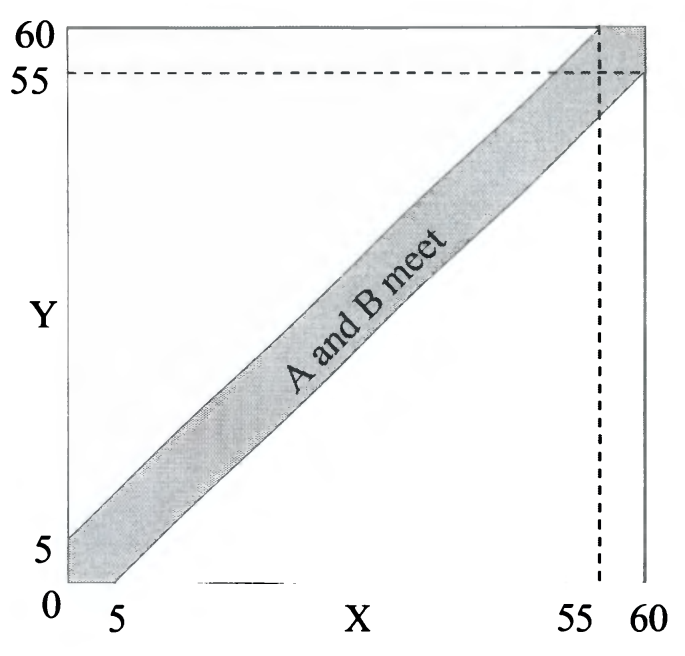
\includegraphics[width=0.5\textwidth]{figures/fig-1.png} % 替换为你的图片文件名
                \caption{Distributions of Banker A's and Banker B's arrival times}
            \end{figure}
        \end{solution}
        \begin{remark}
            subtract \textipa{/s@b"tr\ae kt/}, v. \begin{CJK}{UTF8}{gbsn}减去,扣除\end{CJK}.
        \end{remark}

        \question[](Probability of Triangle) A stick is cut twice randomly (each cut point follows a uniform distribution on the stick), what is the probability that the $3$ segments can form a triangle?
        \begin{solution}
            With loss of generality, we may assume that the length of the stick is $1$. Let $X$ and $Y$ denote the coordinates of the cut points of first and second cuts, respectively. Then both $X$ and $Y$ are uniformly distributed over the interval $[0,1]$, and they are independent. Let $A$ be the event that the $3$ segments can form a triangle. Then we have 
            $$P(A)=P(A,\ X<Y)+P(A,\ X>Y).$$
            \quad If $X<Y$, then the three segments are $X$, $Y-X$ and $1-Y$. They can form a triangle if and only if the following conditions are satisfied:
            \begin{equation*}
               \begin{cases}
                     X+Y-X>1-Y,\\
                     Y-X+1-Y>X,\\
                     X+1-Y>Y-X,
               \end{cases}\Leftrightarrow\begin{cases}
                     Y>\frac{1}{2},\\
                     X<\frac{1}{2},\\
                     2X-2Y+1>0,
               \end{cases}
            \end{equation*}
            which implies that
            $$P(A,X<Y)=P(Y>\frac{1}{2},X<\frac{1}{2},2X-2Y+1>0).$$
            Hence the probability $P(A,X<Y)$ is simply the area of the shadowed region divided by the area of the whole square. 
            \begin{figure}[H]
                \centering
                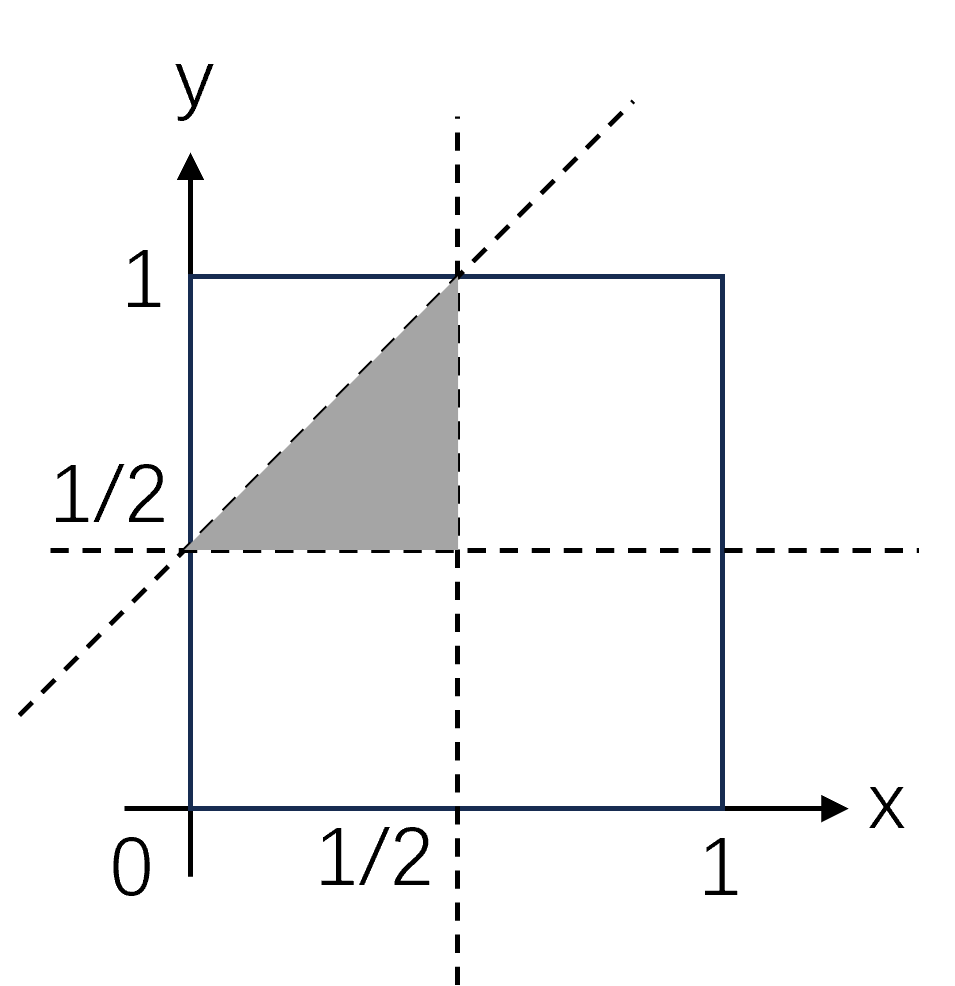
\includegraphics[width=0.5\textwidth]{figures/fig-2.png} % 替换为你的图片文件名
                \caption{Distributions of $X$ and $Y$}
            \end{figure}
            We have
            $$P(A,X<Y)=\frac{1}{8}.$$
            By symmetry, we have
            $$P(A,Y<X)=P(A,X<Y)=\frac{1}{8}$$
            and thus 
            $$P(A)=\frac{1}{4}.$$
        \end{solution}
        \question[](Property of Poisson Process) You are waiting for a bus at a bus station. The buses arrive at the station according to a Poisson process with an average arrival time of $10$ minutes (A = $0.1$/min). If the buses
        have been running for a long time and you arrive at the bus station at a random time, what is your expected waiting time? On average, how many minutes ago did the last bus leave?
        \begin{solution}
            Since the buses form a Poisson process with an average inter-arrival time of $10$ minutes, the waiting-time for the next bus is exponentially distributed with mean $10$. By the memoryless property of the exponential distribution, if we arrive at a random time, our expected waiting time for the next bus is still $10$ minutes. If we look back in time, the memoryless property still applies. So on average, the last bus arrived $10$ minutes ago as well.
        \end{solution}
        \question[](Moments of Normal Distribution) If $X$ follows the standard normal distribution ($X\sim N(0,1)$), what is $\mathbb{E}[X^n]$ for $n=1,2,3,4$?
        \begin{solution}
            The first moment of a distribution is always the expected value. Hence we have $\mathbb{E}[X]=0$. Since the $\mathbb{E}[X]=0$, the second moment of the stand normal distribution is the variance. Hence $\mathbb{E}[X^n]=1$. Note that
            $$\mathbb{E}[X^n]=\int_{-\infty}^{\infty}x^np(x),$$
            where $p(x)$ is the probability density function of $X$. Since $p(x)$ is symmetric about $0$, we know that $\mathbb{E}[X^n]=0$ for any odd positive number $n$.
            
            \quad For $\mathbb{E}[X^4]$, we can use integration by parts. However, to solve $\mathbb{E}[X^n]$ for any integer $n$, the approach using moment generating function may be a better choice. The moment generating function of $X$ is 
            $$M(t)=\mathbb{E}[e^{tX}]=\frac{1}{\sqrt{2\pi}}\int_{-\infty}^{\infty}e^{tx}\cdot e^{-\frac{x^2}{2}}\,{\rm{d}}x=e^{\frac{t^2}{2}}\cdot\frac{1}{\sqrt{2\pi}}\int_{-\infty}^{\infty}e^{-\frac{(x-t)^2}{2}}\,{\rm{d}}x=e^{\frac{t^2}{2}}.$$
            It follows that
            $$M'(t)=te^{\frac{t^2}{2}},$$
            $$M''(t)=e^{\frac{t^2}{2}}+t^2e^{\frac{t^2}{2}},$$
            $$M'''(t)=3te^{\frac{t^2}{2}}+t^3e^{\frac{t^2}{2}},$$
            and 
            $$M^{(4)}(t)=3e^{\frac{t^2}{2}}+6t^2e^{\frac{t^2}{2}}+t^4e^{\frac{t^2}{2}},$$
             which implies that 
        $$\mathbb{E}[X^4]=M^{(4)}(0)=3+6\cdot 0^2+0^4=3.$$
        \quad We can also use the Taylor expansion of $e^{t^2/2}$ at $0$ to compute $\mathbb{E}[X^n]$. We have 
        $$M(t)=e^{\frac{t^2}{2}}=\sum\limits_{n=0}^{\infty}\frac{(2n)!}{2^nn!}\frac{t^{2n}}{(2n)!},$$
        which implies that
        $$\mathbb{E}[X^n]=M^{(n)}(0)=\begin{cases}
            0&\text{if $n$ is odd},\\
            \frac{(n)!}{2^{\frac{n}{2}}(\frac{n}{2})!}&\text{if $n$ is even}.
        \end{cases}$$
        In particular, we have $\mathbb{E}[x^4]=\frac{4!}{2^2\cdot 2!}=3$.
        \end{solution}
    \end{questions}


    \subsection{Expected Value, Variance and Covariance}
    \begin{enumerate}
        \item If $X$ and $Y$ are two independent random variables, then 
        $$E(g(X)h(Y))=E[g(X)]E(h(Y))$$
        for any functions $g$ and $h$.
        \item For any random variables $X$ and $Y$, the covariance of them is defined as 
        $${\rm{Cov}}(X,Y)=\mathbb{E}\Big[(X-\mathbb{E}[X])(Y-\mathbb{E}[Y])\Big]=\mathbb{E}[XY]-\mathbb{E}[X]\mathbb{E}[Y].$$
        It is clear that 
        $${\rm{Cov}}(X,X)={\rm{Var}}(X).$$
        Moreover, if $X$ and $Y$ are independent, then we have ${\rm{Cov}}(X,Y)=0$. However, the converse is not true. Generally, if ${\rm{Cov}}(X,Y)=0$, then $X$ and $Y$ are said to be uncorrelated.

        The correlation coefficient of $X$ and $Y$ are defined as 
        $$\rho(X,Y)=\frac{{\rm{Cov}}(X,Y)}{\sqrt{{\rm{Var}}(X){\rm{Var}}(Y)}}.$$
        Using the Cauchy-Schwarz (\textipa{/SwA:z/}) inequality, we have $|\rho(X,Y)|\le 1$.
        \item Let $X_1$, $X_2$, $\cdots$, $X_n$ be $n$ random variables. Then 
        $${\rm{Var}}\Big(\sum_{i=1}^nX_i\Big)=\sum_{i=1}^n{\rm{Var}}(X_i)+2\sum_{1\le i<j\le n}{\rm{Cov}}(X_i,X_j).$$
        In particular, if $X_1$, $X_2$, $\cdots$, $X_n$ are pairwise uncorrelated/independent, then
        $${\rm{Var}}\Big(\sum_{i=1}^nX_i\Big)=\sum_{i=1}^n{\rm{Var}}(X_i).$$
        \item Let $X$ and $Y$ be two random variables and let $g$ be a function. Then the conditional expected value of $g(X)$ given $Y=y$ is defined by 
        $$\mathbb{E}[g(X)|Y=y]=\begin{cases}
            \sum\limits_x g(x)p_{X|Y}(x|y)&\text{if $X$ is discrete},\\
            \int_{-\infty}^{\infty}g(x)p_{X|Y}(x|y)\,{\rm{d}}x&\text{if $X$ is continuous}.
        \end{cases}$$
        \item (Law of total expectation) Let $X$ and $Y$ be two random variables. Then 
        $$\mathbb{E}[X]=\mathbb{E}[\mathbb{E}[X|Y]]=\begin{cases}
            \sum\limits_y\mathbb{E}[X|Y=y]p(Y=y)&\text{if $Y$ is discrete},\\
            \int_{-\infty}^{\infty}\mathbb{E}[X|Y=y]p_Y(y)\,{\rm{d}}y&\text{if $Y$ is continuous}.
        \end{cases}$$
    \end{enumerate}
    \begin{remark}
        correlate \textipa{/'kO:r@leIt/}, v. \begin{CJK}{UTF8}{gbsn}相互关联\end{CJK}.
    \end{remark}

    \subsubsection{Exercises}
    \begin{questions}
        \question[](Connecting Noodles) You have $100$ noodles in your soup bowl. Being blindfolded, you are told to take two ends of some noodles (each end on any noodle has the same probability of being chosen) in your bowl and connect them. You continue until there are no free ends. The number of loops formed by the noodles this way is stochastic. Calculate the expected number of circles.
        \begin{solution}
            We consider the general case where there are $n$ ($n\ge 1$) noodles. Let $X_n$ be the random variable representing the number of circles formed by the $n$ noodles and let $p_n(k)=P(X_n=k)$ for any $0\le k\le n$. 
            
            \quad It is clear that $p_n(0)=0$. Moreover, the $n$ noodles will ultimately form $n$ loops if and only if, at each step, the two selected ends come from the same noodle. In the first selection, there are a total of $\binom{2n}{2}$ ways to choose two ends, out of which $n$ ways correspond to selecting both ends from the same noodle. In the second selection, there are a total of $\binom{2n-2}{2}$ ways to choose two ends, out of which $n-1$ ways correspond to selecting both ends from the same noodle. Proceeding in this way, we have
            $$P_n(n)=\frac{n(n-1)\cdots 1}{\binom{2n}{2}\binom{2n-2}{2}\cdots\binom{2}{2}}=\frac{2^nn!}{(2n)!}.$$
            \quad Now assume that $n\ge 2$ and $1\le k\le n-1$. Let $Y$ be the event that the first two ends selected come from the same noodle. Then we have $P(Y)=\frac{n}{\binom{2n}{2}}=\frac{1}{2n-1}$. If $Y$ occurs, a cycle is formed and the remaining $n-1$ noodles remain unchanged. It follows that 
            $$P(X_n=k|Y)=P(X_{n-1}=k-1)=p_{n-1}(k-1).$$
            If $Y$ does not occur, then no cycle is formed any two noodles are connected together to form a longer noodle. We may view this longer noodle as a single noodle. It follows that 
            $$P(X_n=k|Y^c)=P(X_{n-1}=k)=p_{n-1}(k).$$
            Applying the law of total probability, we have 
            \begin{align*}
                p_n(k)&=P(X_n=k)\\
                &=P(X_n=k|Y)P(Y)+P(X_n=k|Y^c)P(Y^c)\\
                &=\frac{1}{2n-1}p_{n-1}(k-1)+\frac{2n-2}{2n-1}p_{n-1}(k).
            \end{align*}
            It follows that for any $n\ge 2$, we have 
            \begin{align*}
                \mathbb{E}[X_n]&=\sum\limits_{k=1}^nkp_n(k)\\
                &=\sum\limits_{k=1}^{n-1}\Big(\frac{1}{2n-1}kp_{n-1}(k-1)+\frac{2n-2}{2n-1}kp_{n-1}(k)\Big)+\frac{2^nn!\cdot n}{(2n)!}\\
                &=\frac{1}{2n-1}\sum\limits_{k=1}^{n-1}kp_{n-1}(k-1)+\frac{2n-2}{2n-1}\sum\limits_{k=1}^{n-1}kp_{n-1}(k)+\frac{2^nn!\cdot n}{(2n)!}\\
                &=\frac{1}{2n-1}\sum\limits_{k=1}^{n}kp_{n-1}(k-1)+\frac{2n-2}{2n-1}\sum\limits_{k=1}^{n-1}kp_{n-1}(k)+\frac{2^nn!\cdot n}{(2n)!}-\frac{n}{2n-1}p_{n-1}(n-1)\\
                &=\frac{1}{2n-1}\sum\limits_{k=1}^{n}kp_{n-1}(k-1)+\frac{2n-2}{2n-1}\sum\limits_{k=1}^{n-1}kp_{n-1}(k)\\
                &=\frac{1}{2n-1}\sum\limits_{k=1}^n(k-1)p_{n-1}(k-1)+\frac{1}{2n-1}\sum\limits_{k=1}^np_{n-1}(k-1)+\frac{2n-2}{2n-1}\sum\limits_{k=1}^{n-1}kp_{n-1}(k)\\
                &=\frac{1}{2n-1}\mathbb{E}(X_{n-1})+\frac{1}{2n-1}+\frac{2n-2}{2n-1}\mathbb{E}(X_{n-1})\\
                &=\mathbb{E}(X_{n-1})+\frac{1}{2n-1}.
            \end{align*}
            Using $\mathbb{E}(X_1)=1$ and the above recursion formula, we can compute $\mathbb{E}(X_{100})$.

            \quad It can be seen that the process of deriving the recursive formula for $\mathbb{E}[X_n]$ above is quite complex. Next, we will take a different approach. Consider a random variable $R_n$ following a Bernoulli (\textipa{/b@r"nu:li/}) distribution with parameter $p=\frac{1}{2n-1}$ (that is, $R_n$ takes the value $1$ with probability $\frac{1}{2n-1}$ and the value $0$ with probability $\frac{2n-2}{2n-1}$), which is independent of $X_{n-1}$. Put $Z_n=R_n+X_{n-1}$. Then we can see that
            \begin{align*}
                P(Z_n=n)&=P(R_n=1)P(X_{n-1}=n-1)\\
                &=\frac{1}{2n-1}\cdot\frac{2^{n-1}(n-1)!}{(2n-2)!}\\
                &=\frac{2^nn!}{(2n)!}=p_n(n)
            \end{align*}
            and
            \begin{align*}
                P(Z_n=k)&=P(R_n=1)P(X_{n-1}=k-1)+P(R_n=0)P(X_{n-1}=k)\\
                &\frac{1}{2n-1}p_{n-1}(k-1)+\frac{2n-2}{2n-1}p_{n-1}(k)=p_n(k)\\
                &=p_n(k)
            \end{align*}
            for any $1\le k\le n-1$. Hence $Z_n$ and $X_n$ follow the same distribution and thus
            $$\mathbb{E}[X_n]=\mathbb{E}[Z_n]=\mathbb{E}[R_n]+\mathbb{E}[X_{n-1}]=\frac{1}{2n-1}+\mathbb{E}[X_{n-1}].$$
        \end{solution}
        \begin{remark}
            blindfold \textipa{/"blaIndf@Uld/} n. \begin{CJK}{UTF8}{gbsn}眼罩\end{CJK}. v. \begin{CJK}{UTF8}{gbsn}蒙住眼睛\end{CJK}.
        \end{remark}
        \question[](Optimal Hedge Ratio) You just bought one share of stock A and want to hedge it by shorting stock B. How many shares of B should you short to minimize the variance of the hedged position? Assume that the variance of stock A’s return is $\sigma_A^2$; the variance of B’s return is $\sigma_B^2$; their correlation coefficient is $\rho$.
        \begin{solution}
            Let $r_A$ and $r_B$ be the random variables representing the returns of stock A and stock B, respectively. Suppose that we short $h$ shares of $B$. Then the variance of the hedged position is
            \begin{align*}
                {\rm{Var}}(r_A-hr_B)&={\rm{Var}}(r_A)-2h{\rm{Cov}}(r_A,r_B)+h^2{\rm{Val}}(r_B)\\
                &=\sigma_B^2h^2-2h\rho\sigma_A\sigma_B+\sigma_A^2.
            \end{align*}
            This is a quadratic function of $h$. When $h$ takes the coordinate of the axis of symmetry of its graph, i.e., $-\frac{-2h\rho\sigma_A\sigma_B}{2\sigma_B^2}=\rho\frac{\sigma_A}{\sigma_B}$, the variance of the hedged position is minimized. Hence the optimal hedge ratio is $\rho\frac{\sigma_A}{\sigma_B}$.
        \end{solution}
        \begin{remark}
            hedge \textipa{/hedZ/} v. \begin{CJK}{UTF8}{gbsn}用树篱围住;限制;对冲,采取保值措施以规避风险\end{CJK}. n. \begin{CJK}{UTF8}{gbsn}树篱;防范措施;对冲\end{CJK}.
        \end{remark}
        \begin{remark}
            short v. \begin{CJK}{UTF8}{gbsn}卖空,做空\end{CJK}.
        \end{remark}
        \begin{remark}
            stock \textipa{/stA:k/} n. \begin{CJK}{UTF8}{gbsn}股票\end{CJK}.
        \end{remark}
        \begin{remark}
            position n. \begin{CJK}{UTF8}{gbsn}持仓量,投资头寸\end{CJK}.
        \end{remark}
        \begin{remark}
            hedged position \begin{CJK}{UTF8}{gbsn}对冲后的持仓\end{CJK}.
        \end{remark}
        \begin{remark}
            ratio \textipa{/"reISi@U/} n. \begin{CJK}{UTF8}{gbsn}比率\end{CJK}.
        \end{remark}

        \question[](Dice Game) Suppose that you roll a dice. For each roll, you are paid the face value. Ifa roll gives $4$, $5$ or $6$, you can roll the dice again. Once you get $1$, $2$ or $3$, the game stops. What is the expected payoff of this game?
        \begin{solution}
            Let $X$ be the random variable representing the payoff of this game and let $Y$ be the random variable representing the result of the first roll. For any $i\in\{1,2,3,4,5,6\}$, we have $P(Y=i)=\frac{1}{6}$. If $i\in\{1,2,3\}$, then the distribution of $X$ given $Y=i$ is the degenerate distribution with $X=i$. If $i\in\{4,5,6\}$, then the distribution of the conditional random variable $X|(Y=i)$ coincides with that of $i+X$. In particular, we have $\mathbb{E}[X|Y=i]=i+\mathbb{E}[X]$. Applying the law of total expectation, we have
            \begin{align*}
                \mathbb{E}[X]&=\mathbb{E}\Big[\mathbb{E}[X|Y]\Big]\\
                &=\sum\limits_{i=1}^6\frac{1}{6}\mathbb{E}[X|Y=i]\\
                &=\frac{1+2+3}{6}+\frac{4+\mathbb{E}[X]+5+\mathbb{E}[X]+6+\mathbb{E}[X]}{6}\\
                &=\frac{1}{2}\cdot\mathbb{E}[X]+\frac{7}{2},
            \end{align*}
            which implies that $\mathbb{E}[X]=7$. 
        \end{solution}

        \question[](Card Game) What is the expected number of cards that need to be turned over in a regular $52$-card deck in order to see the first ace?
        \begin{solution}
            We consider the general case where there are $n$ ($n\ge 4$) cards in total, which contains $4$ aces. Let $X_n$ be the random variable representing the number of cards that need to be turned over to see the first ace and let $A$ be the event that the first card turned over is an ace. It is clear that $P(A)=\frac{4}{n}$, $P(X_4=1)=1$ and $\mathbb{E}[X_4]=1$. 
            
            \quad Now assume that $n\ge 5$. If $A$ occurs, then the random variable $X_n|A$ is the degenerate distribution with $X_n|A\equiv 1$, which implies that $\mathbb{E}[X_n|A]=1$. If $A$ does not occur, then it is easy to see that the distribution of $X_n|A^c$ coincides with that of $1+X_{n-1}$. In particular, we have $\mathbb{E}[X_n|A^c]=1+\mathbb{E}[X_{n-1}]$. Applying the law of total expectation, we have
            \begin{align*}
                \mathbb{E}[X_n]&=P(A)\times\mathbb{E}[X_n|A]+P(A^c)\times\mathbb{E}[X_n|A^c]\\
                &=\frac{4}{n}+\frac{n-4}{n}\big(1+\mathbb{E}[X_{n-1}]\big)\\
                &=1+\frac{n-4}{n}\cdot\mathbb{E}[X_{n-1}].
            \end{align*}
            We have $E[X_5]=1+\frac{1}{5}\cdot\mathbb{E}[X_4]=\frac{6}{5}$, $\mathbb{E}[X_6]=1+\frac{2}{6}\cdot\mathbb{E}[X_5]=\frac{7}{5}$ and $\mathbb{E}(X_7)=1+\frac{3}{7}\cdot\mathbb{E}[X_6]=\frac{8}{5}$. By induction, we can show that $\mathbb{E}[X_n]=\frac{n+1}{5}$ for any $n\ge 4$. In particular, we have $\mathbb{E}[X_{52}]=\frac{53}{5}$.
        \end{solution}
        \quad Let's give a different approach.
        \begin{solution}
            There are $4$ aces and $48$ other cards. Let's label the other $48$ cards as $1,2,\cdots,48$. For any $1\le i\le 48$, let $X_i$ be the random variable given by 
            $$X_i=\begin{cases}
                1&\text{if card $i$ is turned over before $4$ aces},\\
                0&\text{otherwise}.
            \end{cases}$$
            Then the total number of cards that need to turned over in order to see the first ace is
            $$X=1+\sum\limits_{i=1}^{48}X_i,$$
            which implies that 
            $$\mathbb{E}[X]=1+\sum\limits_{i=1}^{48}\mathbb{E}[X_i].$$
            By symmetry, these $\mathbb{E}[X_i]$'s are all the same. As shown in the following sequence, card $1$ is equally likely to be in one of the five regions separated by $4$ aces:
            $$\text{$1$\ A\ $2$\ A\ $3$\ A\ $4$\ A\ $5$}$$
            Hence the probability that card $1$ appears before all $4$ aces is $\frac{1}{5}$, which implies that $\mathbb{E}[X_1]=\frac{1}{5}$. It follows that 
            $$E[X]=1+\sum\limits_{i=1}^{48}\mathbb{E}[X_i]=1+\frac{48}{5}=\frac{53}{5}.$$
        \end{solution}
        \begin{remark}
            This is just a special case for random ordering of $m$ ordinary cards and $n$ special cards. The expected position of the first special card is 
            $$1+\sum\limits_{i=1}^m\mathbb{E}[X_i]=1+\frac{m}{n+1}.$$
        \end{remark}
        \begin{remark}
            If the above explanation of the fact $P(X_1=1)=\frac{1}{5}$ is not clear to you, you can consider the following more rigorous proof. We randomly arrange the $52$ cards in a row, and we want card $1$ to be positioned before all $4$ aces. There are $52!$ ways to arrange the $52$ cards. To ensure that card $1$ is placed before all four aces, we first determine the position of card $1$. Since we need to leave at least four spaces for the aces at the end, there are $48$ possible positions for card $1$. If card $1$ is placed in the $i$-th position, then there are $52-i$ positions remaining after it. We then choose four of these positions to place the four aces, which can be done in $A_{52-i}^4$ ways. After placing card $1$ and the four aces, the remaining $47$ cards can be arranged freely in the remaining $47$ positions. Hence the total number of ways to arrange the $52$ cards such that card $1$ is placed before all four aces equals
            $$47!\cdot\sum\limits_{i=1}^{48}A_{52-i}^4=47!\cdot\sum\limits_{i=4}^{51}A_i^4=47!\cdot 4!\cdot\sum\limits_{i=4}^{51}\binom{i}{4}.$$
            Applying the Hockey Stick Identity, we have 
            $$\sum\limits_{i=4}^{51}\binom{i}{4}=\binom{52}{4},$$
            which implies that the total number of ways to arrange the $52$ cards such that card $1$ is placed before all four aces equals
            $$47!\cdot 4!\cdot\binom{52}{4}=\frac{52!}{5}.$$
            Hence the probability that card $1$ is placed before all four aces is $\frac{1}{5}$.
        \end{remark}
        \begin{remark}
            The Hockey Stick Identity states that for any $n\ge k\ge 0$, we have 
            $$\sum\limits_{i=k}^n\binom{i}{k}=\binom{n+1}{k+1}.$$
            Here is a combinatorial interpretation: imagine that you want to choose $k+1$ objects from a set of $n+1$ items. The identity shows that you can count this in another way: consider the largest item selected and suppose it is an position $i+1$ (where $i$ ranges from $k$ to $n$). Then you need to choose the remaining $k$ objects from the first $i$ items, which can be done in $\binom{i}{k}$ ways. Summing over all possible positions $i$ gives the total number of ways, which is exactly $\binom{n+1}{k+1}$.
        \end{remark}
        \begin{remark}
            We can simplify the above argument as follows. First, we choose $5$ positions from the $52$ available positions, which will be occupied by these $5$ key cards. The number of ways to do this is $\binom{52}{5}$. Among these $5$ positions, card $1$ must be placed before all four aces, meaning it must occupy the leftmost (smallest index) position among these $5$ chosen positions. The four aces can be arranged freely in the remaining $4$ positions, and the number of ways to arrange them is $4!$. The remaining $47$ cards can be freely arranged in the remaining $47$ positions, and the number of ways to do this is $47!$. Thus, the total number of favorable arrangements is
            $$\binom{52}{5}\cdot 4!\cdot 47!=\frac{52!}{5},$$
        \end{remark}
        \begin{remark}
            We have another much simpler interpretation of the fact $P(X_1=1)=\frac{1}{5}$. Still, we want to randomly arrange the $52$ cards. We can first arrange the remaining $47$ cards in a sequence. Then, we arrange card $1$ and the four aces separately. Next, we insert these five cards into the sequence of $47$ cards while preserving their original order. Clearly, any arrangement of the $52$ cards can be uniquely obtained through this method. Note that the first step of arranging the $47$ cards and the final step of inserting the five cards while preserving their order do not alter the relative order of these five cards. Therefore, we know that in all possible arrangements of the $52$ cards, the proportion of arrangements where card $1$ appears before the four aces is equal to the proportion of arrangements where card $1$ appears before the four aces in the separate arrangement of the five cards. The latter is clearly $\frac{1}{5}$.
        \end{remark}
        \begin{remark}
            proportion \textipa{/pr@"pO:S@n/} n. \begin{CJK}{UTF8}{gbsn}份额,比例,重要性\end{CJK}.
        \end{remark}

        \question[](Sum of Random Variables) Assume that $X_1$, $X_2$, $\cdots$, $X_n$ are $n$ independent and identically distributed random variables with uniform distribution between $0$ and $1$. What is the probability that $S_n=X_1+X_2+\cdots+X_n\le 1$?
        \begin{solution}
            It is clear that $P(S_n\le 1)$ equals the $n$-dimensional volume of the region 
            $$\Omega_n=\left\{(x_1,\cdots,x_n)\in\mathbb{R}^n:\ 0\le x_i\le 1,\ x_1+x_2+\cdots+x_n\le 1\right\}.$$
            Note that if $x_i\ge 0$ for any $1\le i\le n$, then the condition that $x_i\le 1$ in the definition of $\Omega_n$ is redundant. It is clear that $V(\Omega_1)=1$. Now assume that $n\ge 2$. We have 
            \begin{align*}
                V(\Omega_n)&=\int_{\Omega_n}\,{\rm{d}}x_1\cdots{\rm{d}}x_n\\
                &=\int_0^1\Big(\int_{\substack{x_2,\cdots,x_n\ge 0\\x_2+\cdots+x_n\le 1-x_1}}\,{\rm{d}}x_2\cdots{\rm{d}}x_n\Big)\,{\rm{d}}x_1.
            \end{align*}
            By making the following variable substitution
            $$x_2=(1-x_1)y_2,\quad x_3=(1-x_1)y_3,\quad\cdots,\quad x_n=(1-x_1)y_n,$$
            we obtain that
            \begin{align*}
                V(\Omega_n)&=\int_0^1\Big(\int_{\substack{y_2,\cdots,y_n\ge 0\\y_2+\cdots+y_n\le 1}}(1-x_1)^{n-1}\,{\rm{d}}y_2\cdots{\rm{d}}y_n\Big)\,{\rm{d}}x_1\\
                &=\int_0^1(1-x_1)^{n-1}\Big(\int_{\substack{y_2,\cdots,y_n\ge 0\\y_2+\cdots+y_n\le 1}}\,{\rm{d}}y_2\cdots{\rm{d}}y_n\Big)\,{\rm{d}}x_1\\
                &=\int_0^1(1-x_1)^{n-1}\cdot V(\Omega_{n-1})\,{\rm{d}}x_1\\
                &=V(\Omega_{n-1})\int_0^1(1-x_1)^{n-1}\,{\rm{d}}x_1\\
                &=V(\Omega_{n-1})\times\frac{-1}{n}\cdot(1-x)^{n}\Big|_{0}^1\\
                &=V(\Omega_{n-1})\times\frac{1}{n}.
            \end{align*}
            It follows that $V(\Omega_n)=\frac{1}{n!}$ for any $n\ge 1$. Hence the probability that $S_n\le 1$ is $\frac{1}{n!}$.
        \end{solution}
        \question[](Coupon Collection) There are $N$ distinct types of coupons in cereal boxes and each type, independent of prior selections, is equally likely to be in a box.
        \begin{parts}
            \part If a child wants to collect a complete set of coupons with at least one of each type, how many coupons (boxes) on average are needed to make such a complete set?
            \part If the child has collected $n$ coupons, what is the expected number of distinct coupons?
        \end{parts}
        \begin{solution}
            \begin{parts}
                \part For any $1\le i\le N$, let $X_i$ be the number of additional coupons needed to obtain the $i$-th type after $(i-1)$ distinct types have been collected. Hence the total number of coupons needed is 
                $$X=X_1+X_2+\cdots+X_N.$$
                For any $1\le i\le N$, if $i-1$ distinct types of coupons have already been collected, then a new coupon is of a different type with probability
                $$\frac{1-(i-1)}{N}=\frac{N-i+1}{N}.$$
                It is not difficult to see that the random variable $X_i$ follows a geometric distribution with $p=\frac{N-i+1}{N}$, which implies that 
                $$\mathbb{E}[X_i]=\frac{N}{N-i+1}.$$
                Hence 
                $$\mathbb{E}[X]=\sum\limits_{i=1}^N\mathbb{E}[X_i]=\sum_{i=1}^N\frac{N}{N-i+1}=N(1+\frac{1}{2}+\cdots+\frac{1}{N}).$$
                \part For any $1\le i\le N$, let $Y_i$ be the random variable given by 
                $$Y_i=\begin{cases}
                    1&\text{if the $i$-th type of coupon has been collected},\\
                    0&\text{otherwise}.
                \end{cases}$$
                Then the total number of distinct coupons collected is
                $$Y=Y_1+Y_2+\cdots+Y_N,$$
                By symmetry, we have $\mathbb{E}[Y_1]=\cdots=\mathbb{E}[Y_N]$. For each collected coupon, the probability that it is not of the $i$-th type is $\frac{N-1}{N}$. Since all the $n$ coupons are independent, the probability that none of the $n$ coupons is of the $i$-th type is $(\frac{N-1}{N})^n$. It follows that
                $$\mathbb{E}[Y_1]=P(Y_1=1)=1-P(Y_1=0)=1-(\frac{N-1}{N})^n.$$
                Hence we have 
                $$\mathbb{E}[Y]=\sum\limits_{i=1}^N\mathbb{E}[Y_i]=N\cdot\Big(1-(\frac{N-1}{N})^n\Big).$$
            \end{parts}
        \end{solution}
        \begin{remark}
            coupon \textipa{/"ku:pAn/} n. \begin{CJK}{UTF8}{gbsn}赠券,优惠券\end{CJK}.
        \end{remark}
        \begin{remark}
            cereal \textipa{/"sIri@l/} n. \begin{CJK}{UTF8}{gbsn}谷类食品,谷物植物\end{CJK}. adj. \begin{CJK}{UTF8}{gbsn}谷类的,谷物的\end{CJK}.
        \end{remark}
        \question[](Join Default Probability) If there is a 50\% probability that bond A will default next year and a 30\% probability that bond B will default. What is the range of probability that at least one bond defaults and what is the range of their correlation?
        \begin{solution}
            Let $X$ and $Y$ be the events that $A$ and $B$ default, respectively. Then $P(X)=50\%$ and $P(Y)=30\%$. Since probability is a monotonic increasing function of events, we have
            $$P(X\cup Y)\ge\max\big(P(X),P(Y)\big)=50\%.$$
            We can decompose $X\cup Y$ into two following two disjoint events: $X$ and $Y\setminus X$. By the additivity of probability, we have 
            $$P(X\cup Y)=P(X)+P(Y\setminus X)\le P(X)+P(Y)=80\%.$$
            Hence the range of probability that at least one bond defaults is $[50\%,80\%]$.

            \quad Let $1_X$ and $1_Y$ be the indicator random variables of $X$ and $Y$, respectively. Then we have $\mathbb{E}[1_X]=0.5$, $\mathbb{E}[1_B]=0.3$, ${\rm{Var}}(1_A)=P(X)\times\big(1-P(X)\big)=0.25$ and ${\rm{var}}(1_B)=P(Y)\times\big(1-P(Y)\big)=0.21$. The correlation coefficient of $X$ and $Y$ is
            $$\rho(1_X,1_Y)=\frac{{\rm{Cov}}(1_X,1_Y)}{\sqrt{{\rm{Var}}(1_X){\rm{Var}}(1_Y)}}=\frac{\mathbb{E}[1_X1_Y]-\mathbb{E}[1_X]\mathbb{E}[1_Y]}{\sqrt{{\rm{Var}}(1_X){\rm{Var}}(1_Y)}}.$$
            By definition, we have $\mathbb{E}[1_X1_Y]=P(X\cap Y)$. The range of $P(X\cap Y)$ is $\Big[0,\min\big(P(X),P(Y)\big)\Big]$, i.e., $[0,0.3]$. Hence the range of $\rho(1_X,1_Y)$ is $[-\sqrt{\frac{3}{7}},\sqrt{\frac{3}{7}}]$.
        \end{solution}
        \begin{remark}
            bond \textipa{/ba:nd/} n. \begin{CJK}{UTF8}{gbsn}债券\end{CJK}.
        \end{remark}
        \begin{remark}
            default \textipa{/dI"fO:lt/} v. \begin{CJK}{UTF8}{gbsn}违约\end{CJK}.
        \end{remark}
    \end{questions}

    \subsection{Order Statistics}
    \subsubsection{Key Concept Review}

    \quad Let $X_1$, $X_2$, $\cdots$, $X_n$ be $n$ independent and identically distributed random variables with cumulative distribution function $F(x)$. Put $Y=\min(X_1,X_2,\cdots,X_n)$ and $Z=\max(X_1,X_2,\cdots,X_n)$.

    \quad For any $x\in\mathbb{R}$, we have 
    \begin{align*}
        P(Y\ge x)&=P(X_1\ge x,X_2\ge x,\cdots,X_n\ge x)\\
        &=P(X_1\ge x)P(X_2\ge x)\cdots P(X_n\ge x)\\
        &=\big(1-F(x)\big)^n,
    \end{align*}
    which implies that cumulative distribution function of $Y$ is 
    $$1-\big(1-F(x)\big)^n.$$
    If $F$ is differentiable, then the probability density function of $Y$ is
    $$n\big(1-F(x)\big)^{n-1}F'(x).$$
    \quad Similarly, for any $x\in\mathbb{R}$, we have 
    \begin{align*}
        P(Z<x)&=P(X_1<x,X_2<x,\cdots,X_n<x)\\
        &=P(X_1<x)P(X_2<x)\cdots P(X_n<x)\\
        &=F(x)^n,
    \end{align*}
    which implies that the cumulative distribution function of $Z$ is
    $$F(x)^n.$$
    If $F$ is differentiable, then the probability density function of $Z$ is
    $$nF(x)^{n-1}F'(x).$$

    \subsubsection{Exercises}
    \begin{questions}
        \question[](Expected Value of Max and Min) Let $X_1$, $X_2$, $\cdots$, $X_n$ be IID random variables with uniform distribution between $0$ and $1$. What are the cumulative distribution function, the probability density function and expected value of $Z_n=\max(X_1,\cdots,X_n)$? What are the cumulative distribution function, the probability density function and expected value of $Y_n=\min(X_1,\cdots,X_n)$?
        \begin{solution}
            Let $F(x)$, $p(x)$ denote the cumulative distribution function and probability density function, respectively, of a uniform distribution over the interval $[0,1]$. Then 
            $$p(x)=\begin{cases}
                1&\text{if $0\le x\le 1$},\\
                0&\text{otherwise},
            \end{cases}$$
            and 
            $$F(x)=\begin{cases}
                0&\text{if $x<0$},\\
                x&\text{if $0\le x\le 1$},\\
                1&\text{if $x>1$}.
            \end{cases}$$
            Then the cumulative distribution function of $Z_n$ is
            $$F_Z(x)=F(x)^n=\begin{cases}
                0&\text{if $x<0$},\\
                x^n&\text{if $0\le x\le 1$},\\
                1&\text{if $x>1$},
            \end{cases}$$
            and the probability density function of $Z_n$ is
            $$p_Z(x)=nF(x)^{n-1}p(x)=\begin{cases}
                0&\text{if $x<0$},\\
                nx^{n-1}&\text{if $0\le x\le 1$},\\
                0&\text{if $x>1$}.
            \end{cases}$$
            Hence the expected value of $Z_n$ is
            $$\mathbb{E}(Z_n)=\int_0^1xp_Z(x)\,{\rm{d}}x=\int_0^1nx^n\,{\rm{d}}x=\frac{n}{n+1}.$$
            \quad Moreover, the cumulative distribution function of $Y_n$ is
            $$F_Y(x)=1-\big(1-F(x)\big)^n=\begin{cases}
                0&\text{if $x<0$},\\
                1-(1-x)^n&\text{if $0\le x\le 1$},\\
                1&\text{if $x>1$},
            \end{cases}$$
            and the probability density function of $Y_n$ is
            $$p_Y(x)=\begin{cases}
                0&\text{if $x<0$},\\
                n(1-x)^{n-1}&\text{if $0\le x\le 1$},\\
                0&\text{if $x>1$}.
            \end{cases}$$
            Hence the expected value of $Y_n$ is
            $$\mathbb{E}(Y_n)=\int_0^1xp_Y(x)\,{\rm{d}}x=\int_0^1nx(1-x)^{n-1}\,{\rm{d}}x=\frac{1}{n+1}.$$
        \end{solution}
        \question[](Correlation of Max and Min) Let $X_1$ and $X_2$ be IID random variables with uniform distributions between $0$ and $1$, $Y=\min(X_1,X_2)$ and $Z=\max(X_1,X_2)$. What is the probability of $Y\ge y$ given that $Z\le z$ for any $y,z\in[0,1]$? What is the correlation coefficient of $Y$ and $Z$?
        \begin{solution}
        Let $F(x)$ and $p(x)$ be the cumulative distribution function and probability density function, respectively, of a uniform distribution on $[0,1]$. Then we have
            $$F(x)=\begin{cases}
                0&\text{if $x<0$},\\
                x&\text{if $0\le x\le 1$},\\
                1&\text{if $x>1$},
            \end{cases}$$
            and
            $$p(x)=\begin{cases}
                1&\text{if $0\le x\le 1$},\\
                0&\text{otherwise}.
            \end{cases}$$
            For any $y,z\in[0,1]$, we have 
            \begin{align*}
                P(Y\ge y|z\le z)&=\frac{P(Y\ge y,Z\le z)}{P(Z\le z)}\\
                &=\frac{P(X_1\ge y,X_2\ge y,X_1\le z,X_2\le z)}{P(X_1\le z,X_2\le z)}\\
                &=\frac{P(y\le X_1\le z,y\le X_2\le z)}{P(X_1\le z,X_2\le z)}\\
                &=\frac{P(y\le X_1\le z)P(y\le X_2\le z)}{P(X_1\le z)P(X_2\le z)}\\
                &=\begin{cases}
                    0&\text{if }z\le y,\\
                    \frac{(z-y)^2}{z^2}&\text{if }z>y.
                \end{cases}
            \end{align*}
            It follows that for any $y,z\in[0,1]$, we have
            \begin{align*}
                P(Y\le y,Z\le z)&=P(Z\le z)P(Y\le y|Z\le z)\\
                &=P(Z\le z)\Big(1-P(Y\ge y|Z\le z)\Big)\\
                &=\begin{cases}
                    z^2&\mbox{if }z\le y,\\
                    (2z-y)y&\mbox{if }z>y.
                \end{cases}
            \end{align*}
            It follows that the joint density function of $Y$ and $Z$ is
            $$p(y,z)=\frac{\partial^2P(Y\le y,Z\le z)}{\partial z\partial y}=\begin{cases}
                2&\text{if }0\le y<z\le 1,\\
                0&\text{otherwise}.
            \end{cases}$$
            \quad The cumulative distribution function of $Y$ is
            $$F_Y(y)=1-\big(1-F(y)\big)^2=\begin{cases}
                0&\text{if $y<0$},\\
                1-(1-y)^2&\text{if $0\le y\le 1$},\\
                1&\text{if $y>1$},
            \end{cases}
                $$
            and the probability density function of $Y$ is
            $$
                p_Y(y)=2(1-y)p(y)=\begin{cases}
                    0&\text{if $y<0$},\\
                    2(1-y)&\text{if $0\le y\le 1$},\\
                    0&\text{if $y>1$}.
                \end{cases}
            $$
            Then the cumulative distribution function of $Z$ is 
            $$F_Z(z)=F(z)^2=\begin{cases}
                0&\text{if $z<0$},\\
                z^2&\text{if $0\le z\le 1$},\\
                1&\text{if $z>1$},
            \end{cases}$$
            and the probability density function of $Z$ is
            $$p_Z(z)=2zp(z)=\begin{cases}
                0&\text{if $z<0$},\\
                2z&\text{if $0\le z\le 1$},\\
                0&\text{if $z>1$}.
            \end{cases}$$
            Hence the expected value of $Y$ is
            $$\mathbb{E}(Y)=\int_0^1yp_Y(y)\,{\rm{d}}y=\int_0^12y(1-y)\,{\rm{d}}y=\frac{1}{3},$$
            the expected value of $Z$ is
            $$\mathbb{E}(Z)=\int_0^1zp_Z(z)\,{\rm{d}}z=\int_0^12z^2\,{\rm{d}}z=\frac{2}{3},$$
            the variance of $Y$ is
            $$\text{Var}(Y)=\int_0^1y^2p_Y(y)\,{\rm{d}}y-\mathbb{E}(Y)^2=\int_0^12y^2(1-y)\,{\rm{d}}y-\frac{1}{9}=\frac{1}{18},$$
            and 
            $$\text{Var}(Z)=\int_0^1z^2p_Z(z)\,{\rm{d}}z-\mathbb{E}(Z)^2=\int_0^12z^3\,{\rm{d}}z-\frac{4}{9}=\frac{1}{18}.$$
            \quad Finally, we need to compute the covariance of $Y$ and $Z$. Since 
            $${\rm{Cov}}(X,Y)=\mathbb{E}[YZ]-\mathbb{E}[Y]\mathbb{E}[Z],$$
            it suffices to compute $\mathbb{E}[YZ]$. We have 
            \begin{align*}
                \mathbb{E}[YZ]&=\int_{-\infty}^{\infty}\int_{-\infty}^{\infty}yzp(y,z)\,{\rm{d}}y\,{\rm{d}}z\\
                &=\int_0^1\Big(\int_0^zyzp(y,z)\,{\rm{d}}y\Big)\,{\rm{d}}z\\
                &=2\int_0^1\Big(\int_z^1yz\,{\rm{d}}y\Big)\,{\rm{d}}z=\frac{1}{4},
            \end{align*}
            which implies that 
            $${\rm{Cov}}(X,Y)=\frac{1}{4}-\frac{1}{3}\cdot\frac{2}{3}=\frac{1}{36}$$
            and 
            $$\rho(X,Y)=\frac{{\rm{Cov}}(X,Y)}{\sqrt{{\rm{Var}}(X){\rm{Var}}(Y)}}=\frac{1}{2}.$$
        \end{solution}
        \begin{remark}
            There is an alternative and simpler approach to calculate $\mathbb{E}[YZ]$. Indeed, we always have $YZ=X_1X_2$. Hence $YZ$ and $X_1X_2$ follow the same distribution. It follows that
            $$\mathbb{E}[YZ]=\mathbb{E}[X_1X_2]=\mathbb{E}[X_1]\mathbb{E}[X_2]=\frac{1}{4}$$
            since $X_1$ and $X_2$ are independent.
        \end{remark}
        \begin{remark}
            There is another way to calculate the joint density function of $Y$ and $Z$. Indeed, for any $y,z\in\mathbb{R}$, we have 
            $$P(Y\ge y,Z\le z)=P(Y\ge y,Z\le z,X_1<X_2)+P(Y\ge y,Z\le z,X_1>X_2).$$
            By symmetry, we must have 
            $$P(Y\ge y,Z\le z,X_1<X_2)=P(Y\ge y,Z\le z,X_1>X_2),$$
            which implies that 
            \begin{align*}
                P(Y\ge y,Z\le z)&=2\cdot P(Y\ge y,Z\le z,X_1<X_2)\\
                &=2\cdot P(X_1\ge y,X_2\le z,X_1<X_2)\\
                &=2\cdot P(y\le X_1<X_2\le z).
            \end{align*}
        \end{remark}
        \begin{remark}
            That $Y$ and $Z$ have positive correlation coefficient makes sense, since when $Y$ becomes large, $Z$ tends to becomes as well (note that $Z\ge Y$).
        \end{remark}

        \question[](Random Ants) $500$ ants are randomly put on a $1$-foot string (independent uniform distribution for each ant between $0$ and $1$). Each ant randomly moves toward one end of the string (equal probability to the left or right) at constant speed of $1$ foot/minute until it falls off at one end of the string. Also assume that the size of the ant is infinitely small. When two ants collide head-on, they both immediately change directions and keep on moving at $1$ foot/min. What is the expected time for all ants to fall off the string?
        \begin{solution}
            The difficulty of this problem lies in the fact that when two ants collide, they need to change their directions. However, we can use a clever transformation to avoid this difficulty.

            \quad Please refer to the above diagram. When an ant A collides with another ant B, both of them switch direction. But if we exchange the ants' labels, it is as if the collision never happened: A continues to move to the right and B continues to move to the left. Moreover, after making this equivalent transformation, the total time required remains unchanged, since we are considering the time until the last ant falls off. Hence we can remove the collision rule and consider the ants moving independently.

            \quad Now let $T_1$ denote the time for the first ant to fall off the string, let $D$ denote its initial direction and let $x_0$ be the coordinate of its initial position. Then for any $t\in\mathbb{R}$,
            \begin{enumerate}
                \item if $t\le 0$, then $P(T_1<t)=0$;
                \item if $t\ge 1$, then $P(T_1<t)=1$;
                \item if $0<t<1$, then 
                \begin{align*}
                    P(T_1<t)&=P(D=\text{left})\cdot P(T_1<t|D=\text{left})\\
                    &\quad +P(D=\text{right})\cdot P(T_1<t|D=\text{right})\\
                    &=\frac{1}{2}\cdot P(x_0<t)+\frac{1}{2}\cdot P(x_0>1-t)\\
                    &=\frac{t}{2}+\frac{t}{2}=t.
                \end{align*}
            \end{enumerate}
            Hence $T_1$ also follows that uniform distribution on the interval $[0,1]$ and the problem reduces to calculating the expected value of the maximum of $500$ independent and identically distributed random variables with uniform distribution on $[0,1]$. We know that the probability density function of the maximum is 
            $$p(x)=500x^{499}.$$
            Hence the expected value of the maximum equals
            $$\int_0^1xp(x)\,{\rm{d}}x=\int_0^1x\cdot 500x^{499}\,{\rm{d}}x=\frac{500}{501}.$$
        \end{solution}
        \begin{remark}
            foot n. \begin{CJK}{UTF8}{gbsn}英尺\end{CJK}.
        \end{remark}
        \begin{remark}
            collide \textipa{/k@"laId/} v. \begin{CJK}{UTF8}{gbsn}碰撞\end{CJK}.
        \end{remark}
        \begin{remark}
            collision \textipa{/k@"lIZn/} n. \begin{CJK}{UTF8}{gbsn}碰撞\end{CJK}.
        \end{remark}
    \end{questions}

    \section{Stochastic Process and Stochastic Calculus}

    \subsection{Markov Chain}
    \subsubsection{Key Concept Review}
    \begin{enumerate}
        \item A \textbf{Markov} (\textipa{/"mA:rkO:v/}) \textbf{chain} with state space $S$ is a sequence of infinitely many random variables $X=(X_n)_{n\ge 0}$ taking values in $S$ with the Markov property that given the present state, the future states and the past states are independent:
        \begin{equation}\label{20250213equation1}
            P(X_{n+1}=j|X_n=i,X_{n-1}=i_{n-1},\cdots,X_0=i_0)=P(X_{n+1}=j|X_n=i)
        \end{equation}
        for any $n\in\mathbb{N}$ and any $i_0,i_1,\cdots,i_{n-1},i,j\in S$.
        \item If the probability in equation (\ref{20250213equation1}) does not depend on $n$, then the Markov chain is said to be \textbf{homogeneous}. For a homogeneous Markov chain, the \textbf{transition matrix} $P$ is defined by $(p_{ij})_{i,j\in S}$, where $p_{ij}=P(X_{n+1}=j|X_n=i)$. It is clear that a homogeneous Markov chain is completely determined by its \textbf{initial distribution} $\pi_0$ (the distribution of $X_0$) and its transition matrix $P$.
        \item The transition matrix $P$ satisfies the following properties:
        \begin{enumerate}
            \item $p_{ij}\ge 0$ for any $i,j\in S$;
            \item $\sum_{j\in S}p_{ij}=1$ for any $i\in S$, which implies that the rows of $P$ sum to $1$.
        \end{enumerate}
        Any matrix satisfying these two properties is called a \textbf{stochastic matrix}.
        \item Applying the Markov property, we can calculate \textbf{the probability of any path}:
        $$P(X_1=i_1,X_2=i_2,\cdots,X_n=i_n|X_0=i_0)=p_{i_0i_1}p_{i_1i_2}\cdots p_{i_{n-1}i_n}$$
        for any $i_0,i_1,i_2,\cdots,i_n\in S$.
        \item For any $n\ge 0$ and $i,j\in S$, put $p_{ij}(n)=P(X_n=j|X_0=i)$. Then we have $P^n=(p_{ij}(n))$.
        \item For any stochastic matrix, we can use the \textbf{transition graph} to express it graphically. The vertices of the graph are the states of the Markov chain and there is a directed edge from state $i$ to state $j$ if $p_{ij}>0$. The weight of the edge from $i$ to $j$ is $p_{ij}$.
    \item A state $j\in S$ is called \textbf{accessible} from state $i$ if there is a direction path in the transition graph from $i$ to $j$, i.e., if there exists $n\ge 0$ such that $p_{ij}(n)>0$. Two states $i,,j\in S$ called said to \textbf{communicate} if they are accessible from each other. It is clear that communication is an equivalence relation on $S$. If any two states in $S$ communicate, then the Markov chain is said to be \textbf{irreducible}.
    \item A state $i\in S$ is called \textbf{recurrent} if every state $j$ that is accessible from $i$, $i$ is also accessible from $j$. A state $i\in S$ is called \textbf{transient} (\textipa{/"tr\ae nzI@nt/}, adj. \begin{CJK}{UTF8}{gbsn}转瞬即逝的,短暂的;暂住的\end{CJK}.) if it is not recurrent. It is clear that recurrence and transience are communication classes.
    \item For any state $s\in S$, consider the probability of ever returning to $s$: 
    $$f_{ss}=P(X_n=s\ \text{for some }n\ge 1|X_0=s).$$
    Then 
    $$f_{ss}\begin{cases}
        =1&\text{if $s$ is recurrent},\\
        <1&\text{if $s$ is transient}.
    \end{cases}$$
    Indeed, assume that $s$ is transient, then there exists $j\in S$ such that $p_{sj}(n_0)>0$ for some $n_0\in\mathbb{N}_+$ but $p_{js}(n)=0$ for any $n\in\mathbb{N}_+$. We may assume that $n_0$ is the smallest such integer and claim that for any $n\ge 1$, $P(X_n=s,X_{n_0}=j|X_0=s)=0$. Otherwise, there exists $n_1\ge 1$ such that $P(X_{n_1}=s,X_{n_0}=j|X_0=s)>0$. If $n_1=n_0$, then $P(X_{n_0}=j|X_{n_0}=s)>0$, which is impossible. If $n_1<n_0$, then $P(X_{n_0}=j|X_{n_1}=s)>0$. Using the homogeneity, we have $P_{sj}(n_0-n_1)>0$, which contradicts the minimality of $n_0$. If $n_1>n_0$, then $P(X_{n_1}=s|X_{n_0}=j)>0$. Using the homogeneity, we have $p_{js}(n_1-n_0)>0$, which contradicts the assumption on $j$. Hence for any $n\ge 1$, $P(X_n=s,X_{n_0}=j|X_0=s)<1$, which implies that 
    $$P(X_n=s\ \text{for some }n\ge 1, X_{n_0}=j|X_0=s)=0.$$
    However, by assumption, we have $P(X_{n_0}=j|X_0=s)=p_{sj}(n_0)>0$, which implies that 
    $$P(X_n\ne s\ \text{for any }n\ge 1,X_{n_0}=j|X_{0}=s)>0.$$
    It follows that $P(X_n\ne s\ \text{for any }n\ge 1|X_0=s)>0$, which implies that 
    $$f_{ss}=P(X_n=s\ \text{for some }n\ge 1|X_0=s)<1.$$
    \quad Conversely, assume that 
    $$f_{ss}=P(X_n=s\ \text{for some }n\ge 1|X_0=s)<1.$$
    Then 
    $$P(X_n\ne s\ \text{for any }n\ge 1|X_{0}=s)>0.$$
    We have 
    $$\{X_n\ne s\ \text{for any }n\ge 1\}=\bigcup_{j\in S\setminus\{s\}}\{X_n\ne s\ \text{for any }n\ge 1,\ X_1=j\}.$$
    It follows that 
    there exists $j\in S\setminus\{s\}$ such that 
    $$P(X_n\ne s\ \text{for any }n\ge 1,\ X_1=j|X_0=s)>0.$$
    In particular, we have $p_{sj}=P(X_1=j|X_0=s)>0$.
    \item A state $i\in S$ is called \textbf{absorbing} (\textipa{/@b"zO:bIN/}, v. \begin{CJK}{UTF8}{gbsn}吸收的\end{CJK}.  adj. \begin{CJK}{UTF8}{gbsn}引人入胜的\end{CJK}.) if it is possible to leave this state, i.e., $p_{ii}=1$ and $p_{ij}=0$ for any $j\ne i$.
    \item (\textbf{Equations for absorption probability}) Assume that the state space is $S=\{1,\cdots,M\}$. For any state $i\in S$ that is absorbing or transient, let $a_i$ denote the probability of reaching an absorbing state $s$ starting from state $i$. Then $(a_i)$ is the unique solution to the following system of equations:
    $$
    \begin{cases}
        a_s=1,\\
        a_i=0\ \text{for any absorbing state $i\ne s$},\\
        a_i=\sum\limits_{j=1}^Ma_jp_{ij}\ \text{for any transient state $i$}.
    \end{cases}
    $$
    Why we don't consider the probability of absorption from recurrent states? Because a recurrent state will never visit an absorbing state except itself.
    \item (Equations for the expected time to absorption) For any state $i\in S$ that is absorbing or transient, let $\mu_i$ be the expected time to absorb from state $i$. Then $(\mu_i)$ is the unique solution to the following system of equations:
    \begin{equation}
        \begin{cases}
            \mu_i=0,\ \text{for any absorbing state $i$},\\
            \mu_i=1+\sum\limits_{j=1}^M\mu_jp_{ij},\ \text{for any transient state $i$}.
        \end{cases}
    \end{equation}
    \end{enumerate}

    \subsubsection{Exercises}
    \begin{questions}
        \question[](Gamblers' Ruin Game) Player M has \$1 and player N has \$2. Each game gives the winner \$1 from the other. As a better player, M wins $\frac{2}{3}$ of the games. They play until one of them is bankrupt. What is the probability that M wins?
        \begin{solution}
            We consider the general case where player M begins with $m$ dollars and player N begins with $n$ dollars. Let $p(m,n)$ denote the probability that player M wins given that player M has $m$ dollars and player N has $n$ dollars. Then it is clear that $p(m,0)=1$ and $p(0,n)=0$ for any $m,n\in\mathbb{N}_+$.

            \quad Now assume that $m,n\ge 1$. Consider the first round. Player M wins with probability $\frac{2}{3}$ and loses with probability $\frac{1}{3}$. If player $M$ wins the first round, then player M has $m+1$ dollars and player N has $n-1$ dollars. different rounds are independent., we may regard the game as restarting with M having $m+1$ dollars and N having $n-1$ dollars. Hence given that M wins the first round, the probability that M wins at last is $p(m+1,n-1)$. Similarly, given that M loses the first round, the probability that M wins at last is $p(m-1,n+1)$. Applying the law of total probability, we have 
            $$p(m,n)=\frac{2}{3}p(m+1,n-1)+\frac{1}{3}p(m-1,n+1).$$
            It follows that 
            $$p(1,1)=\frac{2}{3}p(2,0)+\frac{1}{3}p(0,2)=\frac{2}{3},$$
            and 
            $$\begin{cases}
                p(2,1)=\frac{2}{3}p(3,0)+\frac{1}{3}p(1,2)=\frac{2}{3}+\frac{1}{3}p(1,2),\\
                p(1,2)=\frac{2}{3}p(2,1)+\frac{1}{3}p(0,3)=\frac{2}{3}p(2,1),
            \end{cases}$$
            Solving the above system of equations, we have $p(2,1)=\frac{6}{7}$ and $p(1,2)=\frac{4}{7}$. Hence the probability that M wins is $\frac{4}{7}$.
        \end{solution}
        \begin{remark}
            Note that the sum of money of the two players is always $3$. Hence we only need to consider the number of dollars that player M has. In this way, this problem is essentially a one-dimensional random walk with constraints $0$ and $3$.
        \end{remark}
        \begin{remark}
            bankrupt \textipa{/"b\ae \ng kr2pt/} adj. \begin{CJK}{UTF8}{gbsn}破产的\end{CJK}.
        \end{remark}
        \quad We give another approach using the Markov chain, which is essentially the same. The most difficult part of Markov chain problems ofter lies in how to choose the right state space and define the transition probabilities $p_{ij}$'s.
        \begin{solution}
            Define the state space as the possible pairs of dollars that player M and player N have. Then it is clear that the state space is $S=\{(3,0),(2,1),(1,2),(0,3)\}$. Since the sum of the dollars that player M and player N have is always $3$, we only need to consider the number of dollars that player M has. Hence the state space can be simplified as $S=\{0,1,2,3\}$. The initial state is $X_0=1$, the transition matrix is 
            $$
            P=\begin{pmatrix}
               1&0&0&0\\
                \frac{1}{3}&0&\frac{2}{3}&0\\
                0&\frac{1}{3}&0&\frac{2}{3}\\
                0&0&0&1 
            \end{pmatrix},
            $$
            and the transition graph is as follows:
            \begin{figure}[H]
                \centering
                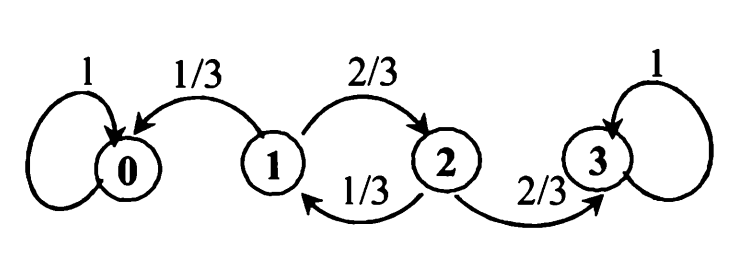
\includegraphics[width=0.5\textwidth]{figures/fig-3.png} % 替换为你的图片文件名
                \caption{Transition graph for Gamblers' ruin problem}
            \end{figure}
            We can see that state $3$ and state $0$ are absorbing states. To calculate the probability that M reaches absorbing state $3$, we can apply the absorption probability equations. For any $i\in S$, let $a_i$ be the absorption probability of reaching absorbing state $3$ starting from state $i$. Then we have
            $$
            \begin{cases}
                a_3=1,\\
                a_0=0,\\
                a_1=\sum\limits_{j=0}^3p_{1j}a_j,\\
                a_2=\sum\limits_{j=0}^3p_{2,j}a_j,
            \end{cases}\Leftrightarrow\begin{cases}
                a_3=1,\\
                a_0=0,\\
                a_1=\frac{1}{3}a_0+\frac{2}{3}a_2,\\
                a_2=\frac{1}{3}a_1+\frac{2}{3}a_3.
            \end{cases}
            $$
            Solving the above system of equations yields $a_1=\frac{4}{7}$ and $a_2=\frac{6}{7}$. Hence the probability that M wins is $\frac{4}{7}$.
        \end{solution}

        \question[](Dice Question) Two players bet on roll(s) of the total of two standard six-face dice. Player A bets that a sum of $12$ will occur first. Player B bets that two consecutive $7$s will occur first. The players keep rolling the dice and record the sums until one player wins. What is the probability that A will win?
        \begin{solution}
            Let $X$ be the event that A wins. Conditioning $P(X)$ on the first throw's sum $F$, we have
            \begin{align*}
                P(X)&=P(X|F=12)P(F=12)+P(X|F=7)P(F=7)\\
                &\quad +P\Big(X|F\not\in\{7,12\}\Big)P\Big(F\not\in\{7,12\}\Big).
            \end{align*}
            Let $(a,b)$ be the result of the first throw. Then
            $$P(F=12)=P(a=6,b=6)=\frac{1}{36},$$
            \begin{align*}
                P(F=7)&=P(a=1,b=6)+P(a=6,b=1)\\
                &\quad + P(a=2,b=5)+P(a=5,b=2)\\
                &\quad + P(a=3,b=4)+P(a=4,b=3)=\frac{6}{36},
            \end{align*}
            and thus 
            $$P(F\not\in\{7,12\})=1-\frac{1}{36}-\frac{2}{36}=\frac{29}{36}.$$
            Therefore, we have 
            \begin{equation}\label{20250213equation8}
                P(X)=\frac{1}{36}P(X|F=12)+\frac{6}{36}P(X|F=7)+\frac{29}{36}P\Big(X|F\not\in\{7,12\}\Big).
            \end{equation}
            \begin{enumerate}
                \item If $F=12$, then A wins, and thus $P(X|F=12)=1$.
                \item If $F\not\in\{7,12\}$, then we may view the game as restarting. Hence
                $$P\Big(X|F\not\in\{7,12\}\Big)=P(X).$$
                \item If $F=7$, then we condition $P(X|F=7)$ on the second throw's sum $G$. We have $P(G=12)=P(F=12)=\frac{1}{36}$, $P(G=7)=P(F=7)=\frac{6}{36}$, and 
                \begin{align*}
                    P(X|F=7)&=P(X|F=7,G=12)P(G=12)\\
                    &\quad +P(X|F=7,G=7)P(G=7)\\
                    &\quad+P\Big(X|F=7,G\not\in\{7,12\}\Big)P\Big(G\not\in\{7,12\}\Big)\\
                    &=\frac{1}{36}P\Big(X|F=7,G=12\Big)+\frac{6}{36}P(X|F=7,G=7)\\
                    &\quad +\frac{29}{36}P(X).
                \end{align*}
                \begin{enumerate}
                    \item If $F=7$ and $G=12$, then A wins, and thus $P(X|F=7,G=12)=1$.
                    \item If $F=7$ and $G=7$, then B wins, and thus $P(X|F=7,G=7)=0$.
                    \item If $F=7$ and $G\not\in\{7,12\}$, then we may view the game as restarting. Hence
                    $$P\Big(X|F=7,G\not\in\{7,12\}\Big)=P(X).$$
                \end{enumerate}
                It follows that 
                $$P(X|F=7)=\frac{1}{36}+\frac{29}{36}P(X).$$
            \end{enumerate}
            \quad Substituting all the conditional probabilities into equation (\ref{20250213equation8}), we have 
            $$P(X)=\frac{1}{36}+\frac{6}{36}\cdot\Big(\frac{1}{36}+\frac{29}{36}P(X)\Big)+\frac{29}{36}P(X),$$
            which implies that $P(X)=\frac{7}{13}$.
        \end{solution}
        \begin{remark}
            consecutive \textipa{/k@n"sekj@tIv/} adj. \begin{CJK}{UTF8}{gbsn}连续的\end{CJK}.
        \end{remark}
        \quad We again provide a Markov chain approach. The key part is still to choose the right state space and define the transition probabilities.
        \begin{solution}
            It is clear that we have the following states: $12$ (A wins) and $7-7$ (B wins), $S$ (starting state) and $7$ (one $7$ occurs, yet no $12$ or $7-7$ occurred). The transition matrix (the row and column indices are sequentially: $12$, $7-7$, $S$ and $7$) is 
            $$
            P=\begin{pmatrix}
                1&0&0&0\\
                0&1&0&0\\
                \frac{1}{36}&0&\frac{29}{36}&\frac{6}{36}\\
                \frac{1}{36}&\frac{6}{36}&\frac{29}{36}&0
            \end{pmatrix},
            $$
            and the transition graph is as follows:
            \begin{figure}[H]
                \centering
                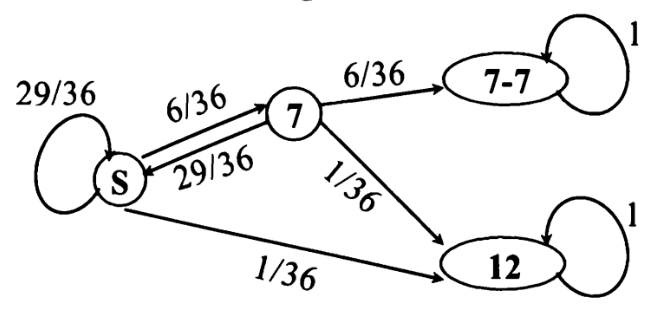
\includegraphics[width=0.5\textwidth]{figures/fig-4.png} % 替换为你的图片文件名
                \caption{Transition graph for Dice question}
            \end{figure}
            \quad It is clear that $12$ and $7-7$ are absorbing states, $S$ and $7$ are transient states. To calculate the probability that A wins, we can apply the absorption probability equations. For any state $i$, let $a_i$ be the absorption probability of reaching state $12$ starting from state $i$. Then we have
            \begin{equation*}
                \begin{cases}
                    a_{12}=1,\\
                    a_{7-7}=0,\\
                    a_S=\sum\limits_{j}p_{Sj}a_j=\frac{1}{36}a_{12}+\frac{29}{36}a_{s}+\frac{6}{36}a_{7},\\
                    a_7=\sum\limits_{j}p_{7j}a_j=\frac{1}{36}a_{12}+\frac{6}{36}a_{7-7}+\frac{29}{36}a_{S}.
                \end{cases}
            \end{equation*}
            Solving the above system of equations yields that $a_S=\frac{7}{13}$.
        \end{solution}
        \question[](Coin Triplets)
        \begin{parts}
        \part If you keep on tossing a fair coin, what is the expected number of tosses such that you can have HHH (heads heads heads) in a row? What is the expected number of tosses to have THH (tails heads heads) in a row?
        \part Keep flipping a fair coin util either HHH or THH occurs in the sequence. What is the probability that you get an HHH subsequence before THH?
        \part Let’s add more fun to the triplet game. Instead of fixed triplets for the two players, the new game allows both to choose their own triplets. Player $1$ chooses a triplet first and announces it; then player $2$ chooses a different triplet. The players again toss the coins until one of the two triplet sequences appears. The player whose chosen triplet appears first wins the game. If both player $1$ and player $2$ are perfectly rational and both want to maximize their probability of winning, would you go first (as player $1$)? If you go second, what is your probability of winning?
        \end{parts}
        \begin{solution}
            \begin{parts}
                \part We use the Markov chain approach. We first consider the question on the expected number of tosses to have HHH in a row. The state space is $$\Omega=\{S,H,HH,HHH\},$$ where $S$ is the starting state, $H$ is the state that one head occurs, $HH$ is the state that only two consecutive heads occur, and $HHH$ is the state that three consecutive heads occur.
                
                \quad If we are in the starting state $S$, the tossing a coin will result in heads with probability $\frac{1}{2}$ and tails with probability $\frac{1}{2}$. The first outcome corresponds to state $H$ while the second outcome corresponds to state $S$ since we can regard the game as restarting. Following a similar analysis, we can obtain the transition matrix, which is (the row and columns indices are sequentially: $S$, $H$, $HH$ and $HHH$)
                $$P=\begin{pmatrix}
                    \frac{1}{2}&\frac{1}{2}&0&0\\
                    \frac{1}{2}&0&\frac{1}{2}&0\\
                    \frac{1}{2}&0&0&\frac{1}{2}\\
                    0&0&0&1
                \end{pmatrix}.$$
                The corresponding transition graph is as follows:
                \begin{figure}[H]
                    \centering
                    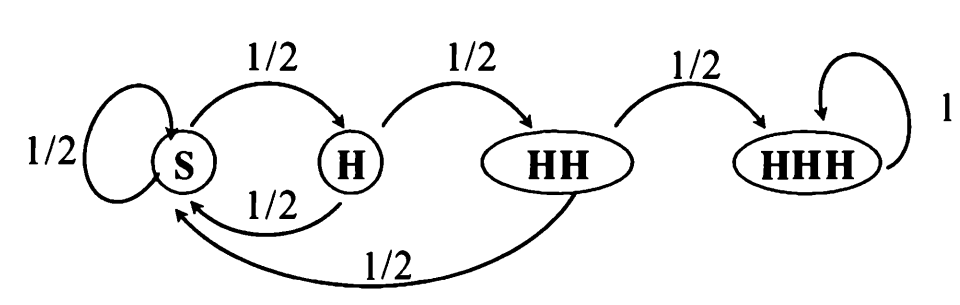
\includegraphics[width=0.6\textwidth]{figures/fig-5.png}
                \end{figure}
                \quad For any state $i\in\Omega$, let $\mu_i$ denote the expected number of tosses to reach state $HHH$ starting from state $i$. Applying the equations for the expected time to absorption, we have 
                $$\begin{cases}
                    \mu_{HHH}=0,\\
                    \mu_{HH}=1+\frac{1}{2}\mu_{S}+\frac{1}{2}\mu_{HHH},\\
                    \mu_{H}=1+\frac{1}{2}\mu_{S}+\frac{1}{2}\mu_{HH},\\
                    \mu_{S}=1+\frac{1}{2}\mu_{S}+\frac{1}{2}\mu_{H}.
                \end{cases}$$
                Solving the above equation yields $\mu_S=14$. Hence the expected number of tosses to have HHH in a row is $14$.

                \quad Next, we consider the question on the expected number of tosses to have THH in a row. The state space is 
                $$\Omega=\{S,T,TH,THH\},$$
                and the transition matrix is (the row and column indices are sequentially: $S$, $T$, $TH$ and $THH$)
                $$P=\begin{pmatrix}
                    \frac{1}{2}&\frac{1}{2}&0&0\\
                    0&\frac{1}{2}&\frac{1}{2}&0\\
                    0&\frac{1}{2}&0&\frac{1}{2}\\
                    0&0&0&1
                \end{pmatrix}.$$
             The transition graph is as follows:
             \begin{figure}[H]
                \centering
                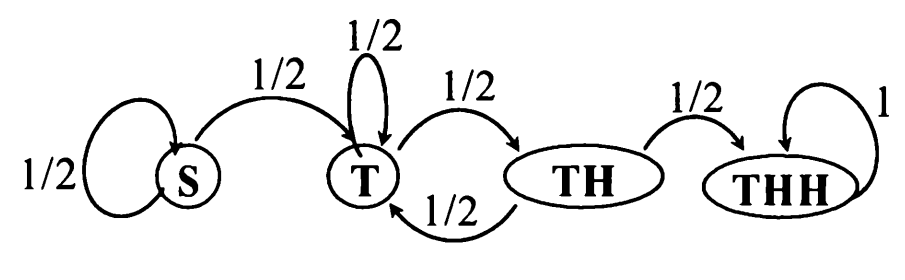
\includegraphics[width=0.6\textwidth]{figures/fig-6.png}
            \end{figure}
            \quad It is clear that $THH$ is the absorbing state. For any $i\in\Omega$, let $\mu_i$ be the expected number of tosses to reach state $THH$ starting from state $i$. Applying the equations for the expected time to absorption, we have 
            \begin{equation*}
                \begin{cases}
                    \mu_{THH}=0,\\
                    \mu_{TH}=1+\frac{1}{2}\mu_{T}+\frac{1}{2}\mu_{THH},\\
                    \mu_{T}=1+\frac{1}{2}\mu_{T}+\frac{1}{2}\mu_{TH},\\
                    \mu_{S}=1+\frac{1}{2}\mu_{S}+\frac{1}{2}\mu_{T}.
                \end{cases}
            \end{equation*}
            Solving the above system of equations yields $\mu_S=8$. Hence the expected number of tosses to have THH is $8$.
            \part The state space is much complicated now, which is 
            $$\Omega=\{S,H,HH,HHH,T,TH,THH\}$$
            and the transition graph is as follows:
            \begin{figure}[H]
                \centering
                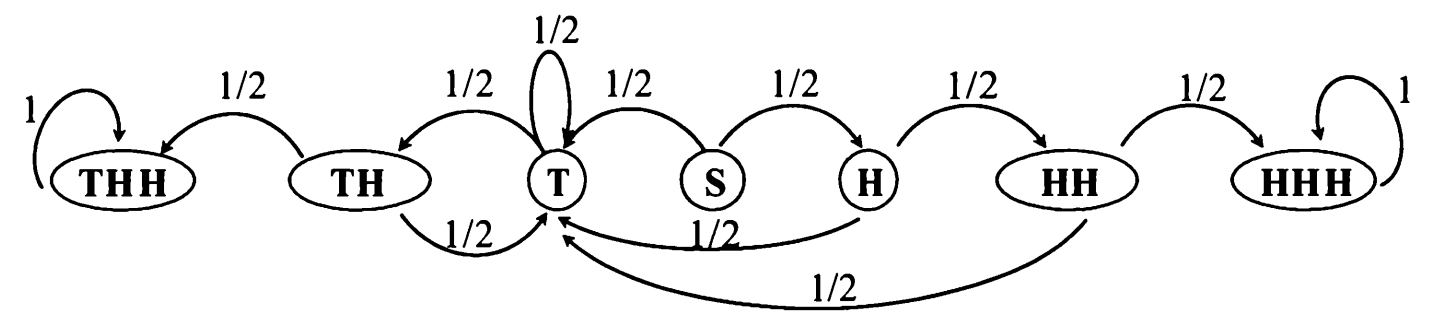
\includegraphics[width=0.8\textwidth]{figures/fig-7.png}
            \end{figure}
            \quad For any state $i\in\Omega$, let $a_i$ be the probability of reaching state $HHH$ before reaching state $THH$ starting from state $i$. Applying the law of total probability, we have 
            $$
            \begin{cases}
                a_{HHH}=1,\\
                a_{THH}=0,\\
                a_S=\frac{1}{2}a_H+\frac{1}{2}a_T,\\
                a_H=\frac{1}{2}a_T+\frac{1}{2}a_{HH},\\
                a_{HH}=\frac{1}{2}a_{T}+\frac{1}{2}a_{HHH},\\
                a_T=\frac{1}{2}a_T+\frac{1}{2}a_{TH},\\
                a_{TH}=\frac{1}{2}a_T+\frac{1}{2}a_{THH}.
            \end{cases}
            $$
            Solving the above system of equations yields 
            \begin{equation*}
                \begin{cases}
                    a_S=\frac{1}{8},\\
                    a_H=\frac{1}{4},\\
                    a_T=0,\\
                    a_{HH}=\frac{1}{2},\\
                    a_{TH}=0.
                \end{cases}
            \end{equation*}
            Hence the probability that we get an HHH subsequence before THH is $\frac{1}{8}$.

            \quad The computational cost of solving this system of equations is relatively high. However, we should have noticed that $a_T=0$. Indeed, once a tail occurs, we will always get THH before HHH, since we need two H to have THH but three H to have HHH. A similar argument applies to $a_{TH}$.
            \part A common misconception is that there is always a best sequence that beats other sequences. This misconception is often founded on a wrong assumption that these sequences are transitive: if sequence A has a higher probability occurring before sequence B and sequence B has a higher probability occurring before sequence C, then sequence A has a higher probability occurring before C. In reality, such transitivity does not exist for this game.
            
            \quad Let's explain why. Let $T_A,T_B,T_C$ be the random variables representing the number of tosses to have sequence A, B and C for the first time, respectively, and assume that $P(T_A<T_B)>\frac{1}{2}$ and $P(T_B<T_C)>\frac{1}{2}$. Then we cannot conclude that $P(T_A<T_C)>\frac{1}{2}$.

            \quad The key point to solve this problem is that no matter what sequence player $1$ chooses, player $2$ can always choose another sequence with a probability of winning higher than $\frac{1}{2}$. Please refer to the following table:
            \begin{figure}[H]
                \centering
                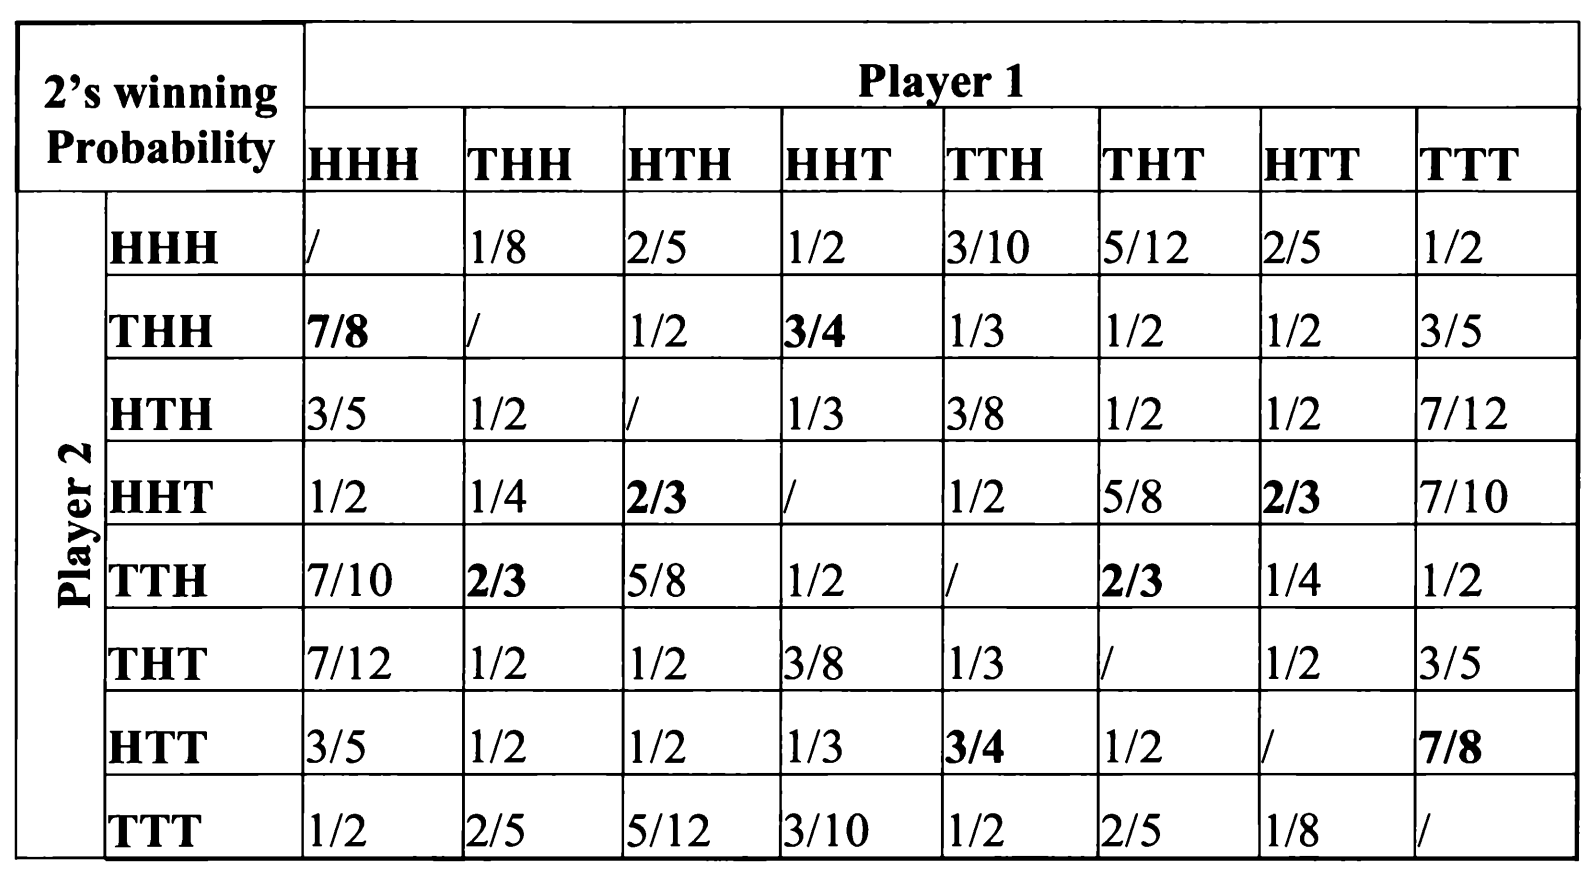
\includegraphics[width=0.9\textwidth]{figures/fig-8.png}\caption{Player $2$'s winning probability with different coin sequence pairs}
            \end{figure}
            \quad As shown in the above table, no matter what triplet player $1$ chooses, player $2$ can always choose another sequence to have better odds of winning. The best sequences that player $2$ can choose in response to player $1$'s choices are highlighted in bold. In order the maximize his odds of winning, player $1$ should choose among HTH, HTT, THH and THT. Even in these cases, player $2$ wins with a probability of $\frac{2}{3}$.
            \end{parts}
        \end{solution}
        \begin{remark}
            triplet \textipa{/"trIpl@t/} n. \begin{CJK}{UTF8}{gbsn}三胞胎\end{CJK}.
        \end{remark}
    \end{questions}
\end{document}